\documentclass{article}
\usepackage[utf8]{inputenc}
\usepackage[default]{raleway}
\usepackage{titlesec, amsmath, comment, tabularx, makecell, listings, array, setspace, geometry, graphicx, xcolor, xparse, fancyvrb, relsize, fancyhdr, booktabs, hyperref}
\usepackage[hypcap=false]{caption}
\usepackage{todonotes}
\usepackage{amsmath}
\usepackage{float}
\usepackage{longtable}
%\geometry{a4paper, left=2cm, right=2cm, top=2cm, bottom=2.5cm}
\renewcommand{\headrulewidth}{0pt}

% Definisci uno stile per i comandi git
\definecolor{light-gray}{gray}{0.92}

\lstdefinestyle{code}{
    frame=single,
    framesep=1mm,
    rulecolor=\color{light-gray},
    backgroundcolor=\color{light-gray},
    basicstyle=\ttfamily,
}
% ----------------------------- Definizione tabella ---------------------------

\newcolumntype{C}[1]{>{\centering\arraybackslash}m{#1}}

%\setcellgapes{2ex} % Imposta l'altezza dell'header (2ex)


% ------------------------------Metadati indice ---------------------------------
\title{\textbf{\fontsize{28}{6}\selectfont Indice}}
\author{\fontsize{14}{6}\selectfont ByteOps}
\date{}

% -----------------------------Creazione footer --------------------------------

\pagestyle{fancy}
\fancyhf{}
\renewcommand{\footrulewidth}{0.4pt} 
\lfoot{
    \parbox[c]{2cm}{
\includegraphics[width=2cm]{../Images/logo.png}}
    \textcolor[RGB]{120, 120, 120}{$\cdot$ Norme di progetto}
}
\rfoot{\thepage}

% --------------------------Modifica formato hyperlinks ------------------------

\hypersetup{
    colorlinks=true,
    linkcolor=black,
    filecolor=black,      
    pdftitle={Norme di Progetto},
    pdfpagemode=FullScreen,
}

% ------------------------------- Valore sotto-paragrafi indice --------------------------------------

\setcounter{secnumdepth}{4}
\setcounter{tocdepth}{4}

\titleformat{\section}
{\normalfont\huge\bfseries}{\thesection}{0.2cm}{}
\titlespacing*{\paragraph}{0pt}{0.5cm}{0.1cm}

\titleformat{\subsection}
{\normalfont\Large\bfseries}{\thesubsection}{0.2cm}{}
\titlespacing*{\paragraph}{0pt}{0.5cm}{0.1cm}

\titleformat{\subsubsection}
{\normalfont\large\bfseries}{\thesubsubsection}{0.2cm}{}
\titlespacing*{\paragraph}{0pt}{0.5cm}{0.1cm}

\titleformat{\paragraph}
{\normalfont\normalsize\bfseries}{\theparagraph}{0.2cm}{}
\titlespacing*{\paragraph}{0pt}{0.5cm}{0.1cm}

% ------------------------------- Front Page ---------------------------------------

\begin{document}
\pagestyle{fancy}
\begin{center}
    
\includegraphics[width = 0.7\textwidth]{../Images/logo.png} \\
    \vspace{0.2cm}
    \textcolor[RGB]{60, 60, 60}{\textit{ByteOps.swe@gmail.com}} \\
    \vspace{2cm}
    \fontsize{16}{6}\selectfont Norme di progetto \\
    \vspace{0.5cm}
\end{center}

\section*{Informazioni documento}
\def\arraystretch{1.2}
\begin{tabular}{>{\raggedleft\arraybackslash}p{0.2\textwidth}|>{\raggedright\arraybackslash}p{0.6\textwidth}c}
    \hline
    \addlinespace
    \textbf{Redattori}      & A. Barutta             \\ & R. Smanio \\ & N. Preto \\ & F. Pozza \vspace{10pt} \\
    \textbf{Verificatori}   & E. Hysa                \\ & L. Skenderi \\ & D. Diotto \vspace{10pt} \\
    \textbf{Destinatari}    & T. Vardanega           \\ & R. Cardin \vspace{10pt} \\
\end{tabular}
\pagebreak

% ------------------------- Changelog ----------------------------
\section*{Registro delle modifiche}
\begin{longtable}{|C{1.5cm}|C{2cm}|C{2cm}|C{2cm}|C{5cm}|}
    \hline
    \textbf{Versione} & \textbf{Data} & \textbf{Autore} & \textbf{Verificatore} & \textbf{Dettaglio} \\
    \hline \hline
    \endhead % Questo comando indica la fine dell'header ripetuto
    
    \label{Git_Action_Version}0.6.0
    & 27/12/2023    & \makecell{D. Diotto}  & N. Preto & \makecell{Completate sezione\\ Metriche di qualità} \\
    \hline
    0.5.1
    & 22/12/2023    & \makecell{R. Smanio}  & A. Barutta & \makecell{Iniziale stesura\\ sezione Metriche\\ di qualità}\\
    \hline
    0.5.0
    & 18/12/2023    & \makecell{R. Smanio}  & D. Diotto & \makecell{Completata sezione\\ Standard per\\ la qualità}\\
    \hline
    0.4.1
    & 10/12/2023    & \makecell{R. Smanio} & N. Preto & \makecell{Prima stesura\\ sottosezioni di\\ Standard per la\\ qualità} \\
    \hline
    0.4.0
    & 05/12/2023    & \makecell{L. Skenderi} & D. Diotto & \makecell{Completate sottosezioni\\ di Processi\\ organizzativi} \\
    \hline
    0.3.2             
    & 04/12/2023    & \makecell{R. Smanio\\ E. Hysa} & D. Diotto & \makecell{Inizio stesura\\ Formazione e\\ aggiornamento Gestione\\ dei Processi} \\
    \hline
    0.3.1             
    & 02/12/2023    & \makecell{L. Skenderi\\ E. Hysa} & D. Diotto & \makecell{Inizio stesura\\ Miglioramento e\\ Gestione dei Processi} \\
    \hline
    0.3.0             
    & 01/12/2023    & \makecell{L. Skenderi\\ E. Hysa} & R. Smanio & \makecell{Completate sottosezioni\\ sezione Processi\\ di supporto} \\
    \hline
    0.2.3
    & 24/11/2023    & \makecell{L. Skenderi\\R. Smanio} & D.Diotto & \makecell{Aggiornate sezioni Gestione\\ della configurazione e\\ Gestione della qualità} \\
    \hline
    0.2.2
    & 22/11/2023    & \makecell{F.Pozza\\R. Smanio} & E. Hysa & \makecell{Iniziale stesura \\ Risoluzione dei problemi\\ delle configurazioni\\ e Gestione \\della qualità} \\
    \hline
    0.2.1
    & 20/11/2023    & \makecell{A. Barutta\\R. Smanio} & E. Hysa & \makecell{Iniziale stesura Gestione\\ delle configurazioni\\ e Joint Review} \\
    \hline
    0.2.0
    & 15/11/2023    & \makecell{F. Pozza\\R. Smanio} & E. Hysa & \makecell{Completate Fornitura,\\ Sviluppo, Verifica e\\ Validazione} \\
    \hline
    0.1.2
    & 10/11/2023    & \makecell{F. Pozza\\A. Barutta} & E. Hysa & \makecell{Aggiornate Fornitura, \\ Sviluppo e \\ inziata sezione Verifica} \\
    \hline
    0.1.1
    & 07/11/2023    & \makecell{F. Pozza\\R. Smanio} & E. Hysa & \makecell{Inzio stesura Fornitura \\ e Sviluppo} \\
    \hline
    0.1.0
    & 05/11/2023    & \makecell{F. Pozza\\R. Smanio} & E. Hysa & \makecell{Sezione Documentazione,\\Introduzione} \\
    \hline
\end{longtable}

\pagebreak

% ------------------------- Generazione automatica indice ----------------------
\setstretch{1.5}
\maketitle
\thispagestyle{fancy}
\tableofcontents
\setstretch{1.2}
\pagebreak


% ---------------------------- Inizio valutazione -------------------------------
\flushleft
\section{Introduzione}

\subsection{Scopo del Manuale}
Il manuale ha lo scopo di assistere l’utente passo dopo passo per un corretto utilizzo del
software così da sfruttarne appieno tutte le funzionalità presenti per offrire un’esperienza
ottimale

\subsection{Glossario}
Incluso nella documentazione è presente il \textbf{\textit{Glossario}} in cui sono definiti tutti i termini specifici o eventualmente ambigui presenti nei vari documenti del progetto. Se un termine è nel \textbf{\textit{Glossario}}, viene segnalato con una \textit{G} a pedice accanto ad esso.

\subsubsection{Raccolta termini del glossario}
Il \textbf{\textit{Glossario}} verrà compilato attraverso un documento condiviso su \LaTeX \textsubscript{\textit{G}}, accessibile a ttti i membri del gruppo. Qui, verranno elencati i ter min  i di particolare rilevanza nel contesto del progetto, seguendo una checklist.   Successivamente, l'\textit{Amministratore} del progetto si occuperà di dettagliare  ulteriormente questi termini nella creazione del \textbf{\textit{Glossario}} ufficiale. 
\subsection{Riferimenti}
\subsubsection{Riferimenti informativi}
    \begin{itemize}
        \item \href {https://www.math.unipd.it/~tullio/IS-1/2023/Progetto/C6.pdf} {Capitolato d'appalto C6 - InnovaCity }
        \item \href{https://www.math.unipd.it/~tullio/IS-1/2023/Dispense/T4.pdf} {Slide del corso di Ingegneria del Software - Gestione di progetto }
        \item \href{https://www.math.unipd.it/~tullio/IS-1/2023/Dispense/T2.pdf} {Slide del corso di Ingegneria del Software - Ciclo di vita del software }
    \end{itemize}
 
\subsubsection{Riferimenti normativi}
    \begin{itemize}
    \item Norme di progetto
    \item \href {https://www.math.unipd.it/~tullio/IS-1/2023/Dispense/PD2.pdf} {Regolamento del progetto didattico }
    \end{itemize}

\vspace{0.5cm}


\section{Processi primari}

\subsection{Sviluppo}

\subsubsection{Introduzione}
L'ISO/IEC 12207:1995 stabilisce le linee guida per il processo di sviluppo, il quale include attività cruciali come analisi, progettazione, codifica, integrazione, testing, installazione e accettazione. È fondamentale svolgere queste attività in stretta aderenza alle linee guida e ai requisiti definiti nel contratto con il cliente, garantendo così un'implementazione accurata e conforme alle specifiche richieste.

\subsubsection{Analisi dei requisiti}
L'analisi dei requisiti è un' attività critica nell'ambito dello sviluppo software poiché stabilisce le basi per il design, l'implementazione e i test del sistema. \\
Secondo lo standard ISO/IEC 12207:1995, lo scopo dell'analisi dei requisiti è di comprendere e definire in modo esaustivo le esigenze del cliente e del sistema. \\
L’attività di analisi richiede di rispondere a domande fondamentali come: “Qual è il dominio?”, “Qual è la cosa giusta da fare?”, "Quali sono le necessità del cliente?" e consiste nella comprensione approfondita del dominio e nella definizione chiara di obiettivi, vincoli e requisiti sia tecnici che funzionali
\paragraph{Obiettivi:}
\begin{itemize}
    \item Definire insieme al proponente gli obiettivi del prodotto per rispecchiarne le aspettative, comprendendo identificazione, documentazione e validazione dei requisiti funzionali e non funzionali;
    \item Facilitare la comprensione comune tra gli stakeholder e il team di sviluppo;
    \item Permettere una stima sulle tempistiche e sui costi;
    \item Fornire ai progettisti requisiti chiari e di facile comprensione;
    \item Favorire l'attività di verifica e test fornendo dei riferimenti pratici.
\end{itemize}

\paragraph{Documentazione}
È compito degli analisti effettuare l'Analisi dei Requisiti, redigendo un documento con il
medesimo nome che deve contenere:
\begin{itemize}
    \item \textbf{Introduzione}: Scopo del documento stesso;
    \item \textbf{Descrizione}: Analisi del prodotto
          \begin{itemize}
              \item Obiettivi del prodotto;
              \item Funzionalità del prodotto;
              \item Caratteristiche utente;
              \item Tecnologie.
          \end{itemize}
    \item \textbf{Casi d'uso}: Funzionalità offerte dal sistema dal punto di vista dell'utente
        \begin{itemize}
            \item Attori: Utenti esterni al sistema;
            \item Elenco dei casi d'uso:
            \begin{itemize}
                \item Casi d'uso in formato testuale;
                \item Diagrammi dei casi d'uso.
            \end{itemize}  
            \item Eventuali diagrammi di attività: permettono di facilitare la comprensione dei processi relativi alle funzionalità.
        \end{itemize}
    \item \textbf{Requisiti}:
        \begin{itemize}
            \item Requisiti funzionali;
            \item Requisiti qualitativi;
            \item Requisiti di vincolo.
        \end{itemize}
\end{itemize}
\paragraph{Casi d'uso}
Forniscono una descrizione dettagliata delle funzionalità del sistema dal punto di vista degli utenti, identificando come il sistema risponde a determinate azioni o scenari. In breve, i casi d'uso sono strumenti utilizzati nell'analisi dei requisiti per catturare e illustrare in modo chiaro e comprensibile come gli utenti interagiranno con il software e quali saranno i risultati di tali interazioni. \\
Ogni caso d'uso e costituito da:
\begin{enumerate}
    \item \textbf{Identificativo} nel formato:\\
          \begin{center}
              \textbf{UC [Numero caso d'uso] . [Numero sotto caso d'uso] - [Titolo]}
          \end{center}
          (ex. UC6.1 - Visualizzazione posizione sensore).\\
          con:
          \begin{itemize}
              \item \textbf{Numero caso d'uso:} ID numerico del caso d'uso;
              \item \textbf{Numero sotto caso d'uso:} ID numerico del sottocaso d'uso (presente esclusivamente se si sta identificando un sottocaso d'uso).
              \item \textbf{Titolo}: Titolo breve ed esplicativo del caso d'uso.
          \end{itemize}
    \item \textbf{Attore principale:} Entità esterna che interagisce attivamente con il sistema per soddisfare una sua necessità;
    \item \textbf{Attore secondario:} Eventuale entità esterna che non interagisce attivamente con il sistema, ma all'interno di un caso d'uso permette al sistema di soddisfare il bisogno dell'attore principale;
    \item \textbf{Descrizione:} Eventuale descrizione breve della funzionalità;
    \item \textbf{Scenario principale:} Sequenza di eventi che si verificano quando un attore interagisce con il sistema per raggiungere l'obbiettivo del caso d'uso (postcondizioni);
    \item \textbf{Estensioni:} Eventuali scenari alternativi che, in seguito ad una o più specifiche condizioni, portano il flusso del caso d'uso a non giungere alle postcondizioni;
    \item \textbf{Precondizioni:} Stato in cui si deve trovare il sistema affinché la funzionalità sia disponibile all'attore;
    \item \textbf{Postcondizioni:} Stato in cui si trova il sistema dopo l'esecuzione dello scenario principale;
    \item \textbf{User story associata:} Breve descrizione di una funzionalità del software, scritta dal punto di vista dell'utente, che fornisce contesto, obiettivi e valore. \\
    Nella forma: "Come [utente] desidero poter [funzionalita] per [valore aggiunto].
\end{enumerate}

\paragraph{Diagrammi dei casi d'uso} 
I diagrammi dei casi d'uso sono strumenti grafici che permettono di visualizzare in modo chiaro e intuitivo le funzionalità offerte dal sistema dal punto di vista dell'utente. Inoltre, consentono di identificare e comprendere rapidamente le relazioni e le interazioni tra i vari casi d'uso, offrendo una visione d'insieme delle funzionalità offerte dal sistema.\\
I diagrammi dei casi d'uso si concentrano sulla descrizione delle funzionalità del sistema dal punto di vista degli utenti senza approfondire dettagli implementativi. La loro finalità principale è quella di evidenziare le interazioni dall'esterno al sistema, offrendo una visione focalizzata sulle funzionalità e sull'interazione dell'utente con il sistema stesso. \\
Un diagramma dei casi d'uso fornisce una panoramica visuale delle interazioni chiave tra gli attori e il sistema, facilitando la comprensione dei requisiti funzionali del sistema e la comunicazione tra gli stakeholder del progetto. \\
Di seguito sono elencati i principali componenti di un diagramma dei casi d'uso:

\begin{itemize}
    \item \textbf{Attori:}
    Gli attori sono le entità esterne al sistema che interagiscono con esso e possono essere utenti umani, altri sistemi software o componenti esterne. \\
    Gli attori sono rappresentati come "stickman" all'esterno del rettangolo che delinea il sistema.
    \begin{minipage}[t]{\linewidth}
        \centering
        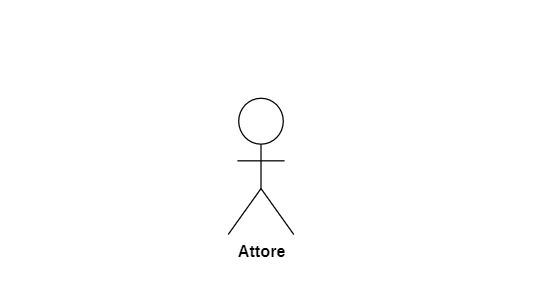
\includegraphics[width=0.6\textwidth]{../Images/NormeDiProgetto/Attore.PNG}
        \captionof{figure}{Rappresentazione Attore}
    \end{minipage}

    \item \textbf{Casi d'Uso:}
    I casi d'uso identificano le diverse funzionalità offerte dal sistema con cui l'attore può interagire. \\
    Ogni caso d'uso viene rappresentato tramite una forma ovale contenente un ID ed un titolo esplicativo.
    \begin{minipage}[t]{\linewidth}
        \centering
        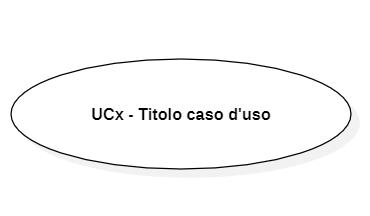
\includegraphics[width=0.6\textwidth]{../Images/NormeDiProgetto/UC.PNG}
        \captionof{figure}{Rappresentazione caso d'uso}
    \end{minipage}

    \item \textbf{Sottocasi d'uso:}
    Un sottocaso d'uso rappresenta una versione più dettagliata di un caso d'uso più generico, offrendo un livello di dettaglio più approfondito sulle funzionalità o sui particolari scenari di utilizzo rispetto al caso d'uso principale.
    \begin{minipage}[t]{\linewidth}
        \centering
        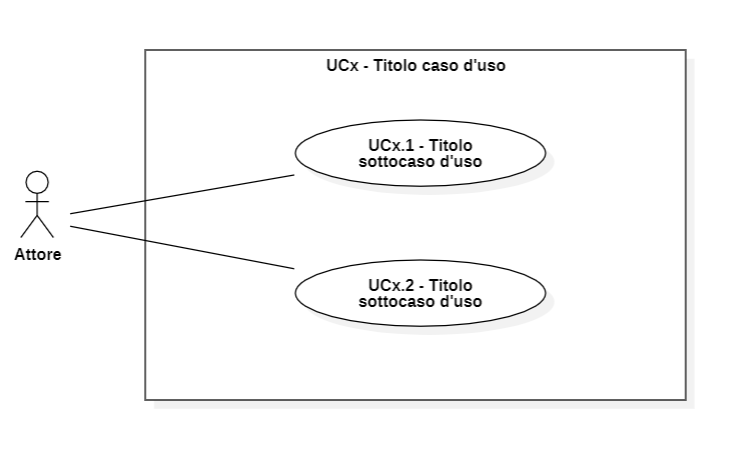
\includegraphics[width=0.6\textwidth]{../Images/NormeDiProgetto/SottocasoD'Uso.PNG}
        \captionof{figure}{Rappresentazione sottocaso d'uso}
    \end{minipage}

    \item \textbf{Sistema:}
    Il sistema viene rappresentato da un rettangolo e viene identificato con un titolo. All'interno del sistema saranno collocati i casi d'uso, mentre al suo esterno gli attori.
    \begin{minipage}[t]{\linewidth}
        \centering
        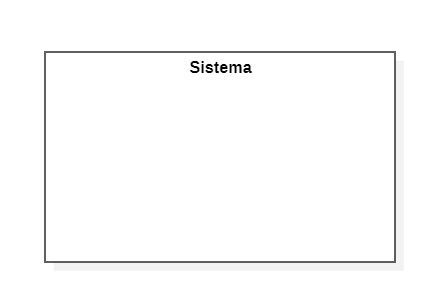
\includegraphics[width=0.6\textwidth]{../Images/NormeDiProgetto/Sistema.PNG}
        \captionof{figure}{Rappresentazione sistema}
    \end{minipage}

    \item \textbf{Relazioni tra Attori e Casi d'Uso:}
    \begin{itemize}
        \item \textbf{Associazione:} \\
        Le linee di associazione collegano gli attori ai casi d'uso corrispondenti, indicando quali attori sono coinvolti in una particolare interazione. Più precisamente, una linea di associazione collega un attore a un caso d'uso quando quell'attore è coinvolto nell'interazione descritta dal caso d'uso stesso. Questo legame rappresenta visivamente il ruolo dell'attore nell'utilizzo o nell'avvio di una funzione specifica offerta dal sistema.
        \begin{minipage}[t]{\linewidth}
            \centering
            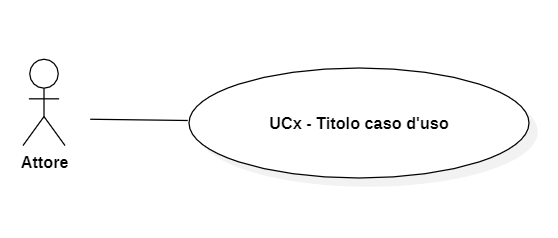
\includegraphics[width=0.6\textwidth]{../Images/NormeDiProgetto/Associazione.PNG}
            \captionof{figure}{Rappresentazione associazione}
        \end{minipage}
    \end{itemize}

    \item \textbf{Relazioni tra attori:}
    \begin{itemize}
        \item \textbf{Generalizzazione tra attori:} \\
        La generalizzazione tra attori rappresenta una relazione di ereditarietà, dove un attore specializzato (figlio) eredita comportamenti e caratteristiche da un attore base (genitore). \\
        Questo aiuta a organizzare gerarchicamente gli attori coinvolti nell'interazione con il sistema nei diagrammi dei casi d'uso. \\
        Viene rappresentata con una linea solida e una freccia vuota (senza testa di freccia) parte dall'attore figlio e arriva all'attore padre.
        \begin{minipage}[t]{\linewidth}
            \centering
            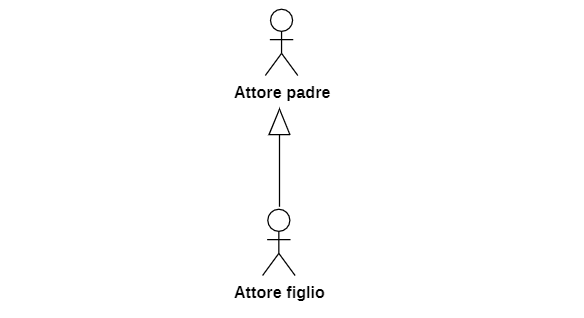
\includegraphics[width=0.6\textwidth]{../Images/NormeDiProgetto/GeneralizzazioneAttori.PNG}
            \captionof{figure}{Rappresentazione generalizzazione tra attori}
        \end{minipage}
    \end{itemize}
    
    \item \textbf{Relazioni tra casi d'uso:}
    \begin{itemize}
        \item \textbf{Inclusione:} \\
        La relazione di inclusione indica che un caso d'uso (detto "includente") include l'esecuzione di un altro caso d'uso (detto "incluso"). \\
        In pratica, quando un attore interagisce con il caso d'uso includente, il caso d'uso incluso viene eseguito come parte integrante del primo. Questo è utile per favorire il riutilizzo e per evitare duplicazione in diversi casi d'uso. \\
        La relazione di inclusione viene rappresentata da una freccia tratteggiata che collega il caso d'uso incluso al caso d'uso che lo include. \\
        Esempio: Supponiamo che per un applicazione e-commerce ci sia un caso d'uso "Conferma ordine". Questo caso d'uso può includere il caso d'uso "Visualizza carrello". Dopo la conferma dell'ordine, l'utente viene automaticamente reindirizzato alla visualizzazione del carrello al fine di ottenere una panoramica completa dei contenuti dell'ordine.
        \begin{minipage}[t]{\linewidth}
            \centering
            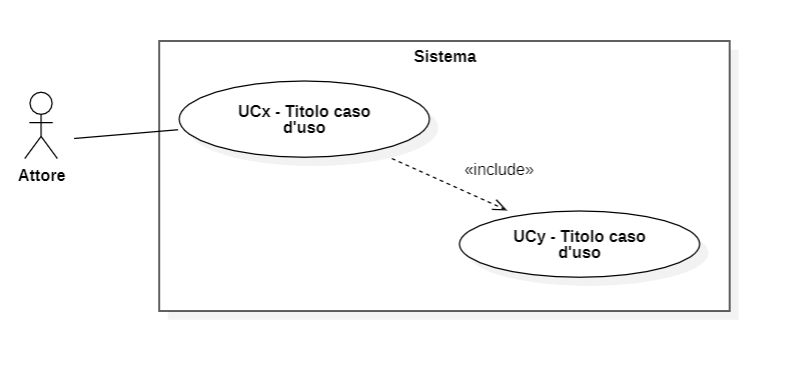
\includegraphics[width=0.6\textwidth]{../Images/NormeDiProgetto/Inclusione.PNG}
            \captionof{figure}{Rappresentazione inclusione}
        \end{minipage}

        \item \textbf{Estensione:} \\
        La relazione di estensione indica che un caso d'uso (detto "estendente") può estendere il comportamento di un altro caso d'uso (detto "esteso") in determinate circostanze. In altre parole, l'esecuzione del caso d'uso estendente può essere estesa o arricchita dal caso d'uso esteso al verificarsi di determinate condizioni. \\
        La relazione di estensione è rappresentata da una freccia tratteggiata che collega il caso d'uso estendente al caso d'uso esteso. \\
        Esempio: Considera un caso d'uso "Visualizzazione errore di autenticazione". Questo caso d'uso potrebbe estendere il caso d'uso "Autenticazione" se durante la fase di autenticazione si inseriscono username e/o password non validi. In questo modo, l'estensione permette di gestire situazioni alternative senza ingombrare lo scenario principale di un caso d'uso e permettendo di evitare duplicazione.
        \begin{minipage}[t]{\linewidth}
            \centering
            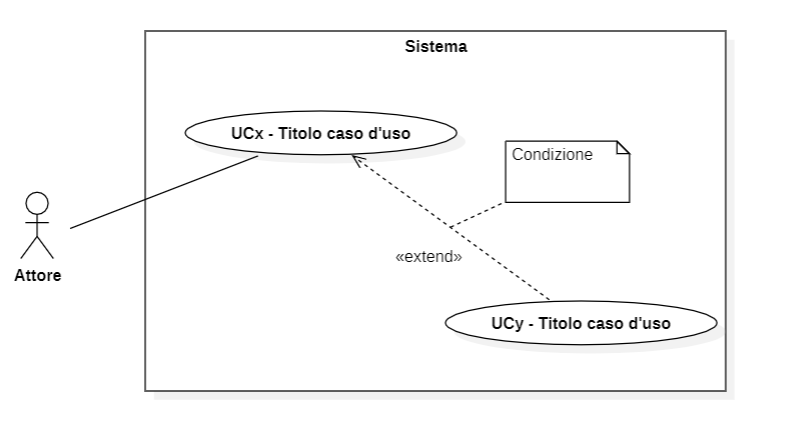
\includegraphics[width=0.6\textwidth]{../Images/NormeDiProgetto/Estensione.PNG}
            \captionof{figure}{Rappresentazione estensione}
        \end{minipage}

        \item \textbf{Generalizzazione casi d'uso:} \\
        La generalizzazione nei diagrammi dei casi d'uso rappresenta una relazione di ereditarietà tra casi d'uso, indicando che un caso d'uso più specifico eredita il comportamento da un caso d'uso più generico. \\
        Questa relazione è simboleggiata da una linea con una freccia vuota che punta dal caso d'uso più specifico al caso d'uso più generico.
        \begin{minipage}[t]{\linewidth}
            \centering
            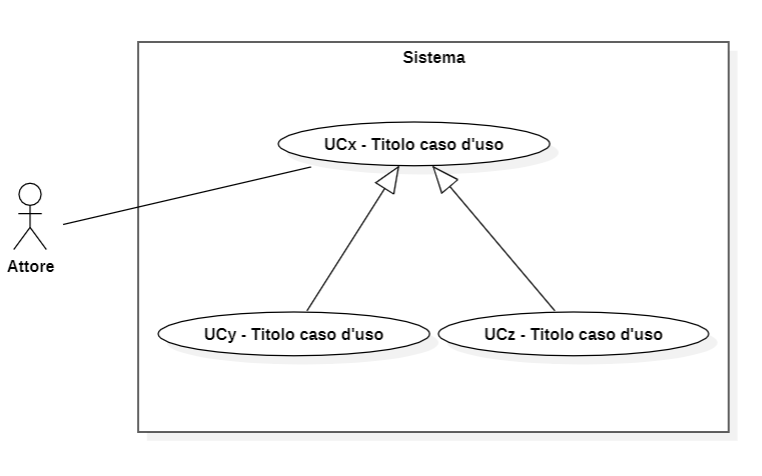
\includegraphics[width=0.6\textwidth]{../Images/NormeDiProgetto/GeneralizzazioneUC.PNG}
            \captionof{figure}{Rappresentazione generalizzazione}
        \end{minipage}
    \end{itemize}

\end{itemize}

\paragraph{Requisiti}
I requisiti di un prodotto software sono specifiche dettagliate e documentate che delineano le funzionalità, le prestazioni, i vincoli e altri aspetti critici che il software deve soddisfare. Questi requisiti fungono da guida per lo sviluppo, il testing e la valutazione del prodotto, assicurando che risponda alle esigenze degli utenti e agli obiettivi del progetto.
Includono
\begin{itemize}
    \item \textbf{Requisiti funzionali:} Descrivono le funzionalità che il software deve avere.
    \item \textbf{Requisiti non funzionali:} Definiscono principalmente criteri di prestazione, qualità, sicurezza e vincoli del sistema, ovvero caratteristiche che non riguardano direttamente le funzionalità specifiche del software.
\end{itemize}
Una precisa definizione dei requisiti è fondamentale: devono risultare inequivocabili e rispondere pienamente alle attese del cliente o del proponente.\\
Ogni requisito è costituito da:
\begin{enumerate}
    \item \textbf{Identificativo} nel formato:\\
          \begin{center}
              \textbf{R [Abbreviazione tipologia requisito] [Codice]}
          \end{center}
          con:
          \begin{itemize}
              \item \textbf{Abbreviazione tipologia requisito:}
                    \begin{itemize}
                        \item \textbf{RF:} Requisito funzionale;
                        \item \textbf{RQ:} Requisito qualitativo;
                        \item \textbf{RV:} Requisito di vincolo;
                    \end{itemize}
              \item \textbf{Codice:} Identificativo progressivo all'interno della tipologia di requisito.
          \end{itemize}
    \item \textbf{Importanza:}
          \begin{itemize}
              \item \textbf{Obbligatorio:} irrinunciabile per qualcuno degli stakeholder;
              \item \textbf{Desiderabile:} non strettamente necessario ma a valore aggiunto;
              \item \textbf{Opzionale:} relativamente utile o contrattabile più avanti nel tempo.
          \end{itemize}
    \item \textbf{Descrizione:} Narrazione chiara e dettagliata che fornisce una spiegazione completa del comportamento o della caratteristica che il software deve possedere;
    \item \textbf{Fonte:} Fonte del requisito (ex. capitolato, Verbale interno/esterno);
    \item \textbf{Casi d'uso:} Elenco casi d'uso associati.
\end{enumerate}
\paragraph{Metriche}
Le metriche nell'analisi dei requisiti sono strumenti utilizzati per valutare, misurare e gestire diversi aspetti dei requisiti di un sistema o di un progetto. Queste metriche aiutano a garantire che i requisiti siano completi, corretti, coerenti e comprensibili.
\begin{table}[h]
    \centering
    \begin{tabular}{|c|c|c|}
    \hline
    Metrica & Nome & Riferimento \\
    \hline \hline
    MROS & Requisiti obbligatori soddisfatti &  \\
    MRDS & Requisiti desiderabili soddisfatti &  \\
    MROPZS & Requisiti opzionali soddisfatti & \\
    \hline
    \end{tabular}
    \caption{Metriche relative all'attività di analisi dei requisiti}
\end{table}

Altri aspetti da valutare per ottenere una specifica dei requisiti ottimale sono:
\begin{itemize}
    \item \textbf{Completezza dei requisiti:} Misura la quantità di requisiti identificati rispetto a quelli effettivamente necessari per il sistema. Una metrica comune è la percentuale di requisiti identificati rispetto a quelli totali;
    \item \textbf{Coerenza:} Valuta la coerenza tra i requisiti. Ad esempio, si potrebbe misurare il numero di conflitti o di requisiti duplicati;
    \item \textbf{Tracciabilità:} Indica la capacità di tracciare i requisiti attraverso le fasi del progetto. Si possono usare metriche come il numero di requisiti tracciati rispetto al totale;
    \item \textbf{Comprensibilità:} Misura la chiarezza e la comprensibilità dei requisiti. Si potrebbe valutare tramite sondaggi o questionari la facilità con cui gli stakeholder comprendono i requisiti;
    \item \textbf{Stabilità:} Misura quanto i requisiti cambiano nel tempo. Si possono usare metriche come il tasso di cambiamento dei requisiti per periodo;
    \item \textbf{Priorità:} Valuta l'importanza relativa dei requisiti. Si possono assegnare punteggi di priorità ai requisiti e valutare la distribuzione di questi punteggi;
    \item \textbf{Testabilità:} Misura la facilità con cui i requisiti possono essere verificati tramite test. Si potrebbe valutare la quantità di requisiti che possono essere testati e quelli che richiedono ulteriori specifiche per la verifica;
    \item \textbf{Misurazione del rischio:} Valuta il livello di rischio associato ai requisiti. Si potrebbero utilizzare valutazioni qualitative o quantitative per attribuire livelli di rischio a ciascun requisito.
\end{itemize}
Ognuna di queste metriche è necessaria ad assicurare che i requisiti siano gestiti in modo efficace e che siano allineati alle esigenze degli stakeholder.

\paragraph{Strumenti}
\begin{itemize}
    \item \textbf{StarUML:}
    È un'applicazione software utilizzata per creare diagrammi e modelli UML nel processo di sviluppo del software. \\
    Aiuta a visualizzare graficamente i vari aspetti di un sistema, consentendo agli utenti di creare e modificare facilmente diagrammi UML come diagrammi dei casi d'uso, delle classi, di attività e altri, semplificando così il processo di progettazione e analisi dei sistemi software.
\end{itemize}

\subsubsection{Progettazione}

\paragraph{Scopo}
Lo scopo primario dell'attività di progettazione consiste nell'identificare una soluzione realizzativa ottimale che soddisfi appieno le esigenze di tutti gli stakeholder, considerando i requisiti e le risorse disponibili. \\
La progettazione risponde alla domanda chiave: 'Qual è il modo migliore per realizzare ciò di cui c'è bisogno?'. \\
È cruciale definire l'architettura del prodotto prima di avviare la fase di codifica, perseguendo correttezza per costruzione piuttosto che correttezza per correzione. Questo approccio permette di gestire in modo efficiente la complessità del prodotto, garantendo una struttura robusta e coesa durante l'intero processo di sviluppo. \\
L'obiettivo principale è quindi quello di assicurare il soddisfacimento dei requisiti attraverso un sistema di qualità delineato dall'architettura del prodotto. Questo comporta:
\begin{itemize}
    \item Identificare parti componibili conformi ai requisiti, dotate di specifiche chiare e coese, sviluppandole con risorse sostenibili e costi contenuti;
    \item Organizzare il sistema in modo da agevolare adattamenti futuri;
    \item Gestire la complessità del sistema attraverso una progettazione dettagliata, suddividendo il sistema in unità architetturali per semplificare la codifica di ciascuna parte, rendendola facilmente gestibile, veloce e verificabile.
\end{itemize}

\paragraph{Obiettivi}
Inizialmente, il team di progettazione condurrà un'analisi approfondita per selezionare con attenzione le tecnologie più adatte, valutandone attentamente i punti di forza, le debolezze e le eventuali criticità. \\
Una volta individuate le tecnologie appropriate, si procede allo sviluppo di un'architettura di alto livello per comprendere e delineare la struttura generale del prodotto, costituendo così una base di partenza per la realizzazione del PoC.
Questa architettura fornisce una visione panoramica del sistema, identificando i principali componenti, i flussi di dati e le interazioni tra di essi. Si presterà particolare attenzione a rendere il sistema flessibile e adatto a potenziali modifiche future. \\
Successivamente, si avvierà lo sviluppo di un Proof of Concept (PoC), parte fondamentale della Technology Baseline, per valutare le decisioni prese riguardo all'architettura e alle tecnologie adottate, nonché per verificarne l'aderenza agli obiettivi e alle specifiche del progetto. \\
In seguito allo sviluppo e ad un'attenta analisi del POC, si procederà con iterazioni aggiuntive, apportando miglioramenti, aggiustamenti e aggiunte, fino a giungere a un design completo. Questo design sarà fondamentale per lo sviluppo dell'MVP (Minimum Viable Product), che costituirà una versione essenziale e funzionale del prodotto e che sarà parte della Product Baseline.

\paragraph{Documentazione}
\textbf{Specifica tecnica} \\
Il documento descrive in modo approfondito il design definitivo del prodotto e fornisce istruzioni precise agli sviluppatori, guidandoli nella corretta implementazione della soluzione software secondo i requisiti e le specifiche indicate. Ciò permette di ridurre la complessità e le ambiguità nel processo di sviluppo del software, contribuendo a garantire che il prodotto finale sia allineato alle aspettative del cliente e funzioni in modo ottimale.
Questo documento comprende diversi elementi cruciali: 
\begin{itemize}
    \item \textbf{Tecnologie utilizzate}: Specifica le tecnologie e le librerie di terze parti integrate nel sistema;
    \item \textbf{Architettura logica}: Definisce i componenti, i ruoli, le connessioni e le interazioni nel sistema;
    \item \textbf{Architettura di deployment}: Indica come le componenti architetturali vengono allocate e distribuite nel sistema in esecuzione;
    \item \textbf{Pattern architetturali e design pattern}: Descrive i design pattern architetturali adottati e quelli influenzati dalle tecnologie utilizzate, oltre agli eventuali idiomi a livello più basso;
    \item \textbf{Vincoli e linee guida}: Include restrizioni e regole da seguire durante lo sviluppo;
    \item \textbf{Procedure di testing e validazione}: Indica i processi per testare e verificare che il software soddisfi i requisiti specificati;
    \item \textbf{Requisiti tecnici}: Specifica in dettaglio i requisiti prestazionali, di sicurezza, di scalabilità e di compatibilità con determinate piattaforme che il software deve soddisfare
\end{itemize}

\paragraph{Qualità dell'architettura}
\begin{itemize}
    \item \textbf{Sufficienza}: L'architettura soddisfa i requisiti funzionali e non funzionali definiti per il software, senza sovradimensionamento o sottodimensionamento;
    \item \textbf{Comprensibilità}: La chiarezza e la facilità con cui è possibile comprendere l'architettura software, rendendo agevole per gli sviluppatori e gli stakeholder capire come funziona il sistema;
    \item \textbf{Modularità}: L'architettura è suddivisa in moduli o componenti chiaramente definiti, consentendo la separazione delle responsabilità e facilitando la manutenzione, l'aggiornamento e lo sviluppo parallelo;
    \item \textbf{Robustezza}: La capacità del software di gestire situazioni anomale o errate senza interruzioni gravi o perdite di dati, mantenendo un funzionamento accettabile;
    \item \textbf{Flessibilità}: La facilità con cui il sistema può essere adattato o esteso per soddisfare nuovi requisiti o cambiamenti senza richiedere modifiche radicali o strutturali;
    \item \textbf{Riusabilità}: La capacità di riutilizzare parti del software in contesti diversi, riducendo lo sforzo di sviluppo e migliorando l'efficienza;
    \item \textbf{Efficienza}: Il software utilizza in modo ottimale le risorse disponibili, come memoria e CPU, per eseguire le sue funzioni nel minor tempo possibile;
    \item \textbf{Affidabilità}: La capacità del software di svolgere correttamente le sue funzioni in modo coerente e prevedibile nel tempo;
    \item \textbf{Disponibilità}: Il software è accessibile e operativo quando richiesto, riducendo al minimo i tempi di inattività non pianificati;
    \item \textbf{Sicurezza rispetto a malfunzionamenti (Safety)}: La prevenzione di danni fisici o danni a persone o beni a causa di malfunzionamenti del software;
    \item \textbf{Sicurezza rispetto a intrusioni (Security)}: La protezione del software da accessi non autorizzati, manipolazioni e intrusioni esterne;
    \item \textbf{Semplicità}: La capacità di mantenere l'architettura software il più semplice possibile senza compromettere la funzionalità o l'efficacia;
    \item \textbf{Incapsulazione}: Il nascondere dei dettagli implementativi all'esterno di un componente, consentendo l'accesso solo attraverso un'interfaccia definita;
    \item \textbf{Coesione}: La misura in cui i componenti all'interno di un modulo o un'unità funzionano insieme per un obiettivo comune senza essere eccessivamente interdipendenti;
    \item \textbf{Basso accoppiamento}: Il grado di dipendenza tra i diversi moduli o componenti del software, cercando di minimizzare le interazioni o le dipendenze tra di essi per migliorare la manutenibilità e la flessibilità del sistema.
\end{itemize}

\paragraph{Diagrammi UML}
Vantaggi:
\begin{itemize}
    \item \textbf{Chiarezza nella comunicazione}: Rendono più comprensibili e chiari i concetti tecnici ai team e agli stakeholder;
    \item \textbf{Standardizzazione}: Offrono un linguaggio comune per la documentazione e la comprensione dei sistemi software;
    \item \textbf{Analisi e progettazione visiva}: Aiutano a identificare errori e lacune nel progetto prima dell'implementazione;
    \item \textbf{Modellazione e simulazione}: Consentono la creazione di modelli predittivi, riducendo rischi e costi durante lo sviluppo;
    \item F\textbf{acilitano la manutenzione}: Semplificano la comprensione della struttura del software, agevolando le operazioni di manutenzione;
    \item \textbf{Riducono errori di progettazione}: Aiutano a individuare problemi prima dell'implementazione, riducendo correzioni costose;
    \item \textbf{Supportano la documentazione}: Offrono una guida visiva per comprendere il sistema, inclusa nella documentazione del progetto.
\end{itemize}

A supporto dell'attività di progettazione verranno utlizzati i \textbf{Diagrammi delle classi}. \\

\paragraph*{Diagrammi delle classi}
Ciascun diagramma delle classi rappresenta le proprietà e le relazioni tra le varie componenti di un sistema, offrendo una prospettiva statica e non a run time.
Le classi sono rappresentate graficamente sotto forma di rettangoli divisi in tre sezioni:
\begin{enumerate}
    \item \textbf{Nome della classe}: Identificativo della classe. \\
    È rappresentato in grassetto seguendo la convenzione PascalCase e deve esplicitare chiaramente la responsabilità della classe. Se la classe è astratta, il nome viene scritto in corsivo.
    \item \textbf{Attributi}: Ogni elemento sarà presentato in una riga separata, secondo il seguente formato: \\
    \begin{center}\texttt{Visibilità Nome: Tipo [Molteplicità] = Valore/i di Default}\end{center}
    \begin{itemize}
        \item \textbf{Visibilità}: precede obbligatoriamente ogni attributo e rappresenta uno dei seguenti indicatori:
        \begin{itemize}
            \item $-$ : Visibilità privata;
            \item $+$ : Visibilità pubblica;
            \item $\#$ : Visibilità protetta;
            \item $\sim$ : Visibilità di package;
        \end{itemize}
        \item \textbf{Nome}: Rappresenta univocamente l'attributo. Dev'essere rappresentativo dell'attributo e deve seguire la notazione \texttt{nomeAttributo: tipo}. \\
        Qualora l'attributo fosse di tipo costante, allora il nome verrà scritto interamente in maiuscolo \texttt{NOMEATTRIBUTO: tipo};
        \item \textbf{Molteplicità}: Nel caso di una sequenza di elementi, come liste o array, la sua lunghezza può essere specificata con la sintassi \texttt{tipoAttributo[molteplicità]}. \\
        Se la sequenza contiene un numero di elementi non conosciuto a priori, verrà adottata la sintassi \texttt{tipoAttributo[*]}. \\
        Nel caso di un singolo elemento, la sua dichiarazione è opzionale.
        \item \textbf{Default}: Ogni attributo può essere dichiarato con un valore di default.
    \end{itemize}
    \item \textbf{Firme dei metodi}: Descrivono il comportamento delle classi individuate. Ogni metodo occuperà una riga e seguiranno il formato: \\
    \begin{center} \texttt{Visibilità Nome (Parametri Formali): Tipo di Ritorno} \end{center}
    \begin{itemize}
        \item \textbf{Visibilità}: Segue la convenzione definita per gli attributi.
        \item \textbf{Nome}: Rappresenta l'identificativo univoco del metodo e descrive in modo esplicito il suo obiettivo, seguendo la notazione \textit{PascalCase}.
        \item \textbf{Parametri formali}: Il loro numero varia da $0$ a $n$ e sono separati tramite la virgola. Ogni parametro seguirà la notazione e le convenzioni definite per gli attributi.
        \item \textbf{Tipo di ritorno}: Determina il tipo che verrà ritornato dal metodo.
    \end{itemize}
    I metodi getter, setter e i costruttori non verranno inclusi fra i metodi. \\
    I metodi astratti verrano scritti in corsivo. \\
    I metodi statici verranno sottolineati. \\
    L'assenza di attributi o metodi in una classe, determinerà una visualizzazione di campi vuoti nel diagramma delle classi.
\end{enumerate}

I diagrammi delle classi sono collegati tra loro mediante frecce che delineano le rispettive relazioni di dipendenza. \\
Qui di seguito, saranno delineate le rappresentazioni mediante frecce per le diverse relazioni: \\
\begin{itemize}
    \item \textbf{Dipendenza}: Se la classe A utilizza servizi, metodi o membri forniti dalla classe B, si dice che la classe A dipende dalla classe B e tale relazione viene rappresentata con una freccia tratteggiata dalla classe A alla classe B. \\
    La relazione di dipendenza indica il minor grado di accoppiamento tra due classi: un cambiamento nella classe B può influenzare la classe A, ma non viceversa.
    \begin{figure}[H]
        \centering
        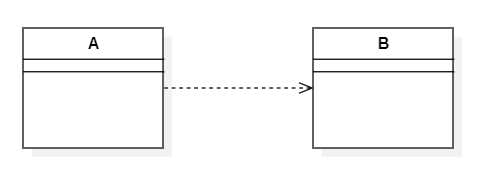
\includegraphics[width=0.6\textwidth]{../Images/NormeDiProgetto/ClassDiagram_Dipendenza.PNG}
        \caption{Diagramma delle classi di una relazione di Dipendenza.}
    \end{figure}
    \item \textbf{Associazione}: L'associazione tra due classi viene rappresentata tramite una linea continua e orientata. Questa connessione indica che la classe A contiene campi o istanze della classe B. \\
    Le molteplicità di occorrenza possono essere espresse tramite valori posizionati agli estremi della freccia:
    \begin{itemize}
        \item $\mathbf{0...1}$: A può possedere 0 o 1 istanza di B;
        \item $\mathbf{0...*}$: A può possedere 0 o più istanze di B;
        \item $\mathbf{1}$:  A possiede esattamente un'istanza di B (in questo caso non è necessario specificare la molteplicità);
        \item $\mathbf{*}$: A possiede più istanze di B;
        \item $\mathbf{n}$: A possiede esattamente n istanze di B.
    \end{itemize}
    \begin{figure}[H]
        \centering
        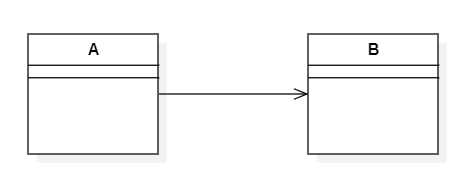
\includegraphics[width=0.6\textwidth]{../Images/NormeDiProgetto/ClassDiagram_Associazione.PNG}
        \caption{Diagramma delle classi di una relazione di Associazione.}
    \end{figure}
    \item \textbf{Aggregazione}: Rappresentata con una freccia a diamante vuota. \\
    Indica una relazione "parte di" (part of) in cui una classe è composta da diverse parti (altre classi), ma le parti possono esistere anche indipendentemente dalla classe principale. Nella figura la classe B è parte della classa A.
    \begin{figure}[H]
        \centering
        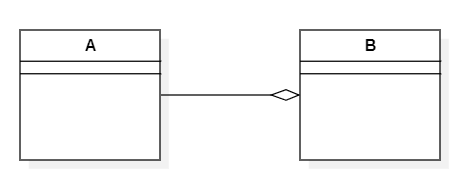
\includegraphics[width=0.6\textwidth]{../Images/NormeDiProgetto/ClassDiagram_Aggregazione.PNG}
        \caption{Diagramma delle classi di una relazione di Aggregazione.}
    \end{figure}
    \item \textbf{Composizione}: Rappresentata con una freccia a diamante piena. È simile all'aggregazione, ma le parti (altre classi) sono strettamente dipendenti dalla classe principale e non possono esistere indipendentemente. \\
    Nella figura la classe B è parte della classe A ed esiste solo come parte di A.
    \begin{figure}[H]
        \centering
        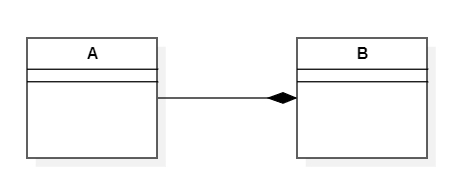
\includegraphics[width=0.6\textwidth]{../Images/NormeDiProgetto/ClassDiagram_Composizione.PNG}
        \caption{Diagramma delle classi di una relazione di Composizione.}
    \end{figure}
    \item \textbf{Generalizzazione}: Rappresentata con una freccia continua vuota. Rappresenta la relazione "is a" (è un) tra una classe genitore (superclasse) e una classe figlia (sottoclasse). La classe figlia eredita attributi e comportamenti dalla classe genitore. \\
    Equivale all'ereditarietà nei linguaggi di programmazione. \\
    Le proprietà della superclasse non si riportano nel diagramma della sottoclasse, a meno di override.
    \begin{figure}[H]
        \centering
        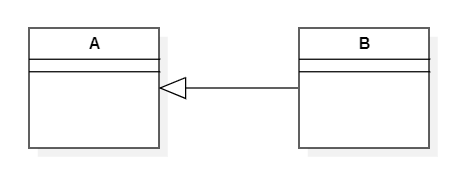
\includegraphics[width=0.6\textwidth]{../Images/NormeDiProgetto/ClassDiagram_Generalizzazione.PNG}
        \caption{Diagramma delle classi di una relazione di Generalizzazione.}
    \end{figure}
    \item \textbf{Interface Realization}: La relazione di "interface realization" indica che una classe fornisce l'implementazione dei metodi definiti in un'interfaccia specifica. Questa relazione è importante quando si desidera mostrare come una classe concreta soddisfi i requisiti di un'interfaccia specifica definendo e implementando i suoi metodi. \\
    Nella figura l'interfaccia A, rappresentata tramite un cerchio, viene implementata dalla classe B e questa relazione viene rappresentata graficamente con una linea da B ad A.
    \begin{figure}[H]
        \centering
        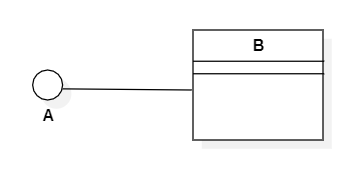
\includegraphics[width=0.6\textwidth]{../Images/NormeDiProgetto/InterfaceRealization.PNG}
        \caption{Diagramma delle classi di una relazione di Interface Realization.}
    \end{figure}
\end{itemize}

\paragraph{Design Pattern}
I design pattern costituiscono una risposta consolidata a problemi di progettazione che si presentano ciclicamente in determinati contesti. Questi modelli offrono un approccio di progettazione riusabile, garantendo qualità nella soluzione ed una rapida implementazione.
L'adozione di un design pattern avviene soprattutto quando una soluzione si è dimostrata efficace in un contesto specifico. Solitamente vengono fornite guide dettagliate sull'applicazione dei pattern, delineando il loro utilizzo ottimale.
Ogni design pattern deve essere accompagnato da una rappresentazione grafica illustrativa del suo funzionamento, da una spiegazione testuale della sua logica e da una descrizione della sua utilità all'interno dell'architettura complessiva. Questa documentazione svolge un ruolo chiave nel favorire una comprensione approfondita dell'integrazione del design pattern nell'architettura generale e nella prevenzione di errori di progettazione.

\paragraph{Test}
Nell'ambito del processo di sviluppo, il testing riveste un ruolo fondamentale nell'assicurare la qualità del prodotto finale. Durante questa fase, si delineano i requisiti di testing, si definiscono i casi di test e i criteri di accettazione, fungendo da strumenti per valutare il software. \\
Il suo obiettivo principale è individuare e risolvere eventuali problemi o errori presenti nel software prima del rilascio del prodotto finale. In aggiunta, il processo di testing è essenziale per garantire che il software soddisfi le specifiche e le aspettative del cliente. \\
I progettisti avranno il completo controllo di questa attività, compresa la definizione dei test da eseguire. Inoltre, nella sezione x.y.z, si può trovare una descrizione dettagliata delle varie tipologie di test e della terminologia da adottare, offrendo così un'ulteriore chiarezza su questa fase critica del processo di sviluppo del software.

\paragraph{Metriche}
\begin{table}[H]
    \centering
    \begin{tabular}{|c|c|c|}
    \hline
    Metrica & Nome & Riferimento \\
    \hline \hline
    MAC & Accoppiamento tra classi &  \\
    MATC & Attributi per classe &  \\
    MPM & Parametri per metodo & \\
    MLCM & Linee di codice per metodo &  \\ 
    \hline
    \end{tabular}
    \caption{Metriche relative all'attività di progettazione}
\end{table}

\paragraph{Strumenti}
\begin{itemize}
    \item \textbf{StarUML:}
    È un'applicazione software utilizzata per creare diagrammi e modelli UML nel processo di sviluppo del software. \\
    Aiuta a visualizzare graficamente i vari aspetti di un sistema, consentendo agli utenti di creare e modificare facilmente diagrammi UML come diagrammi dei casi d'uso, delle classi, di attività e altri, semplificando così il processo di progettazione e analisi dei sistemi software.
\end{itemize}

\subsubsection{Codifica}
\paragraph{Scopo}
L'attività di codifica è affidata al programmatore e rappresenta il momento cruciale in cui le funzionalità richieste dal proponente prendono forma. \\
Durante questa fase, le idee e i concetti delineati dai progettisti vengono tradotti in codice, creando istruzioni e procedure che i calcolatori possono eseguire. \\
I programmatori devono rispettare scrupolosamente le linee guida e le norme stabilite per garantire che il codice sia in linea con le specifiche stabilite e che traduca in modo accurato le concezioni iniziali dei progettisti.
\paragraph{Aspettative}
La codifica è finalizzata alla creazione di un prodotto software in linea con le richieste del committente e conforme agli accordi stipulati.\\
Il rigoroso rispetto delle norme garantisce la creazione di codice di alta qualità, facilitando la manutenzione, l'estensione e la verifica del software, contribuendo costantemente al miglioramento della sua qualità complessiva.
\paragraph{Norme di codifica}
Le seguenti norme sono state formalizzate prendendo spunto dal libro "Clean Code" di Robert C. Martin.

\paragraph*{Nomi significativi}
Usare nomi che riflettano il significato e lo scopo delle variabili, funzioni e classi. Evitare abbreviazioni ambigue.
\paragraph*{Indentazioni e formattazione consistente}
L'utilizzo di un tab per ciascun livello di annidamento è fondamentale per assicurare una struttura coerente del codice, migliorandone la comprensione e agevolandone la gestione.
\paragraph*{Lunghezza dei metodi}
La lunghezza ottimale dei metodi può variare a seconda del contesto e delle best practices di programmazione. Tuttavia, in generale, molti esperti consigliano che i metodi siano brevi e focalizzati su una singola responsabilità.
Un principio comune è quello espresso da Robert C. Martin nel suo libro "Clean Code", che suggerisce che i metodi dovrebbero essere idealmente lunghi quanto basta per svolgere una singola operazione e non più lungo di quanto si possa visualizzare senza dover scorrere la pagina. \\
Questo favorisce:
\begin{itemize}
    \item \textbf{Chiarezza};
    \item \textbf{Manutenibilità};
    \item \textbf{Comprensibilità};
    \item \textbf{Testabilità:} Metodi più brevi sono più facili da testare in isolamento, il che favorisce l'implementazione di test di unità efficaci;
    \item \textbf{Conformità ai principi SOLID:} La brevità dei metodi è spesso correlata al principio Single Responsibility Principle (SRP) dei principi SOLID, il che favorisce la costruzione di codice più modulare e coeso.
\end{itemize} 

\paragraph*{Lunghezza righe di codice}
Mantenere le righe di codice entro i 80-120 caratteri permette una migliore leggibilità del codice su schermi di diverse dimensioni e facilita la visualizzazione di più file affiancati.
Inoltre, limitare la lunghezza delle righe può incoraggiare la scrittura di codice più chiaro e modulare.
\paragraph{Commenti}
Evitare commenti superflui e non necessari: l'obiettivo è scrivere il codice in modo chiaro e autoesplicativo, riducendo la dipendenza da commenti esplicativi. 
\subsubsection{Configurazione dell'ambiente di esecuzione}
\paragraph{Docker}

La progettazione dei Docker e la scrittura dei Dockerfile sono considerate parte del processo di sviluppo del software.
Le regole e le best practice di codifica per i file Docker sono fondamentali per garantire la creazione, la gestione e la distribuzione efficace dei container:
\begin{itemize}
    \item \textbf{Chiarezza e Coerenza:}
    \begin{itemize}
        \item Utilizzare nomi descrittivi per le immagini e i container.
        \item Mantenere una struttura coerente e consistente per assicurare un'organizzazione uniforme all'interno dei file Docker.
    \end{itemize}

\item \textbf{Versionamento:}
    \begin{itemize}
        \item Specificare sempre la versione dell'immagine di base (base image) per garantire la riproducibilità.
        \item Evitare di utilizzare tag "latest" per immagini di produzione.
    \end{itemize}

\item \textbf{Minimizzazione degli strati (Layering):}
    \begin{itemize}
        \item Ridurre il numero di istruzioni nell'esecuzione del Dockerfile per minimizzare gli strati dell'immagine.
        \item Raggruppare le istruzioni correlate per sfruttare la cache Docker.
    \end{itemize}

\item \textbf{Sicurezza:}
    \begin{itemize}
        \item Utilizzare immagini ufficiali o verificate.
        \item Evitare di eseguire processi Docker con privilegi elevati quando possibile.
        \item Usare ARG per parametrizzare informazioni sensibili.
    \end{itemize}

\item \textbf{Ottimizzazione delle risorse:}
    \begin{itemize}
        \item Limitare l'uso di risorse all'interno dei container (CPU, memoria, etc.).
        \item Usare immagini leggere e ottimizzate per la produzione.
    \end{itemize}

\item \textbf{Gestione delle variabili d'ambiente:}
    \begin{itemize}
        \item Usare variabili d'ambiente per configurazioni dinamiche.
        \item Fornire valori predefiniti opportuni per le variabili d'ambiente.
    \end{itemize}

\item \textbf{Logging e monitoraggio:}
    \begin{itemize}
        \item Configurare i container per registrare i log in modo efficace.
        \item Integrare strumenti di monitoraggio, se necessario.
    \end{itemize}

\item \textbf{Pulizia e riduzione delle dimensioni:}
    \begin{itemize}
        \item Pulire i pacchetti temporanei e le risorse non necessarie dopo l'installazione delle dipendenze.
        \item Ridurre le dimensioni delle immagini utilizzando multi-stage builds.
    \end{itemize}

\item \textbf{Documentazione:}
    \begin{itemize}
        \item Aggiungere commenti nel Dockerfile per spiegare le decisioni di progettazione.
        \item Fornire una documentazione chiara su come utilizzare e configurare il container.
    \end{itemize}

\item \textbf{Testing:}
    \begin{itemize}
        \item Implementare test automatizzati per il Dockerfile e i container, se possibile.
    \end{itemize}
\end{itemize}
\paragraph{Strumenti}
\begin{itemize}
    \item \textbf{VSCode}
    \item \textbf{Docker}
    \item \textbf{Git}
\end{itemize}



\section{Processi di supporto}

\subsection{Documentazione}

\subsubsection{Introduzione}
La documentazione costituisce l'insieme di informazioni scritte che accompagnano un prodotto software, fornendo dettagli utili a sviluppatori, distributori e utenti.\\
Tra gli scopi della documentazione troviamo:
\begin{itemize}
    \item Comprensione del prodotto senza supporto umano, usandola come mezzo di comunicazione;
    \item Segnare il confine tra creatività e disciplina;
    \item Assicurare che i processi produttivi si svolgano con la qualità attesa.
\end{itemize}
L'obiettivo della sezione è:
\begin{itemize}
    \item  Definire delle procedure ripetibili che permettano di uniformare la documentazione prodotta dal gruppo ed il metodo di lavoro;
    \item  Raccogliere ed organizzare le norme che i membri del team devono seguire così da semplificare l'operazione di scrittura dei documenti.
\end{itemize}
Tali norme dovranno essere applicate da tutti i membri del team, ed i sorgenti \LaTeX\ che contengono tale documentazione verranno inseriti nel repository disponibile all'indirizzo:
\href{https://github.com/ByteOps-swe/Sorgente-documenti}{https://github.com/ByteOps-swe/Sorgente-documenti}

\begin{comment} \paragraph*{Primi approcci alla redazione di documenti e problematiche riscontrate}
Per la composizione iniziale dei documenti richiesti per la candidatura, è stato sperimentato un'approccio che impiegava gli strumenti di Google Drive. Tale metodologia consentiva ai redattori di redigere agevolmente i documenti senza la necessità di padroneggiare la sintassi LaTeX, con l'intenzione di trasporre successivamente il contenuto in LaTeX una volta che fosse stato validato dai verificatori. Tuttavia, questo approccio ha suscitato problematiche, tra cui:
\begin{itemize}
    \item Rischio di incoerenza tra il contenuto presente negli strumenti di Google Drive.
    \item Prolungato impiego di tempo per la riscrittura in LaTeX, dovuto alla necessità di un passaggio aggiuntivo.
\end{itemize}
Per tali ragioni si è presa la decisione di adottare un nuovo approccio.
\end{comment}
\paragraph{Documentation as Code}\label{sec:DocumentationAscode}
L'approccio che si intende adottare è quello di "Documentation as Code" (Documentazione come Codice) che consiste nel trattare la documentazione di un progetto software allo stesso modo in cui si tratta il codice sorgente. Questo approccio è incentrato sull'utilizzo di pratiche e strumenti tipici dello sviluppo software per creare, gestire e distribuire la documentazione.
Alcuni aspetti chiave di "Documentation as Code" includono:
\begin{itemize}
    \item \textbf{Versionamento}
    \item \textbf{Scrittura in Formato Testuale}
    \item \textbf{Automazione}
    \item \textbf{Collaborazione}
    \item \textbf{Integrazione Continua}
    \item \textbf{Distribuzione}
\end{itemize}
Questo approccio porta diversi vantaggi, tra cui una maggiore coerenza, una migliore tracciabilità delle modifiche e facilità di manutenzione. Inoltre, il concetto di "Documentation as Code" si allinea con la filosofia DevOps, dove la collaborazione e l'automazione sono valori chiave.\\

\subsubsection{Sorgente documenti}
Poiché i documenti vengono redatti in LaTeX, per favorire una migliore collaborazione tra diversi autori, si è scelto di creare un file sorgente per ciascuna sezione e sottosezione di ogni documento. Questo approccio consente a ciascun autore di lavorare sulle singole sezioni o sottosezioni, evitando di apportare modifiche a parti del documento non pertinenti al proprio ambito. Infine, si creerà un file principale che prenderà il nome del documento, nel quale verranno collegati tutti i file delle varie sezioni e sottosezioni mediante l'uso del comando \verb|\input{Sezione.tex}| o, nel caso delle sottosezioni, \verb|\input{Sottosezione.tex}|.
Nel caso dei Verbali, essendo documenti composti da sezioni molto brevi, non si utilizza questo approccio.

\subsubsection{Ciclo di vita dei documenti}
Il ciclo di vita dei documenti è una sequenza di stati e attività:
\begin{enumerate}
    \item \textbf{Stato: Necessità}
          \begin{enumerate}
              \item Nasce la necessità di una documentazione, per obbligo o per opportunità;
              \item Pianicazione della sua stesura;
              \item Suddivisione in sezioni;
              \item Durante le riunioni, si procede alla discussione e alla definizione collettiva di una traccia per il contenuto;
              \item Assegnazione delle sezioni ai redattori tramite task su ITS.
          \end{enumerate}
    \item \textbf{Stato: Redazione}
          \begin{enumerate}
              \item  Ogni tipo di documento viene creato secondo la struttura specificata nei prossimi paragrafi;
              \item Il team realizza il documento redigendone il contenuto rispettando le norme definite;
          \end{enumerate}
    \item \textbf{Stato: Verifica}
          \begin{enumerate}
              \item Quando completato il documento viene revisionato dai verificatori;
              \item Il documento viene compilato e il PDF generato viene inserito nella repository all'indirizzo: \href{https://github.com/ByteOps-swe/Documents} {https://github.com/ByteOps-swe/Documents} ;
          \end{enumerate}
    \item \textbf{Stato: Manutenzione}
          \begin{enumerate}
              \item Manutenzione: ogni documento sotto configuration management deve essere modificato in accordo alle norme di versionamento e di change management.
              \item La richiesta di modifica nasce da una nuova necessità sul contenuto del documento e riporta il documento allo stato omonimo.
          \end{enumerate}
\end{enumerate}

%\textbf{Procedimento in sintesi}\\
%   Per rispettare i principi  di "Documentation as Code" l'approccio attualmente adottato richiede la competenza e l'utilizzo di LaTeX per la stesura dei documenti e una repository ad accesso limitato Git chiamata "Sorgente documenti" dove versionarli. I redattori, seguendo la struttura dettagliata nei prossimi paragrafi, redigeranno il contenuto dei documenti utilizzando il linguaggio \LaTeX\ su un ramo dedicato nella repository "Sorgente documenti". \\
%  Al termine del loro lavoro, segnaleranno il completamento posizionando l'Issue relativa al compito di redazione nella colonna "Da revisionare" della \href{https://github.com/orgs/ByteOps-swe/projects/1/views/1}{DashBoard documentazione} di GitHub (unica e condivisa sia dalla repository pubblica "\href{https://github.com/ByteOps-swe/Documents}{Documents}" che dalla repository "Sorgente documenti") e generando una pull request . Questa colonna conterrà i compiti relativi ai documenti completati dai redattori, che necessitano ora della validazione da parte dei verificatori. \\

% I file sorgenti LaTeX saranno quindi gestiti e versionati nella repository con accesso limitato denominata "Sorgente documenti", strutturata in modo identico alla repository pubblica chiamata "\href{https://github.com/ByteOps-swe/Documents}{Documents}" ma con file \LaTeX\ al posto dei PDF. \\
%   I verificatori quindi troveranno il documento da validare in questa repository quando riceveranno una notifica mail generata dalla pull request.\\
%  Quando i verificatori avranno convalidato il contenuto, dovranno seguire le istruzioni al paragrafo ~\ref{sec:verificatori} per formalizzare la verifica.


\paragraph{I redattori}

Il redattore responsabile della redazione di un documento o di una sua sezione deve seguire lo stesso approccio richiesto per la codifica del software, adottando il workflow noto come "feature branch".\\
\vspace{0.1cm}
\textbf{Caso redazione nuovo documento, sezione o modifica}\\
Dalla repository  "Sorgente documenti" contenente i sorgenti \LaTeX, il redattore dovrà creare un nuovo branch Git in locale e passare ad esso mediante l'utilizzo del comando:
\begin{lstlisting}[style=code]
    git checkout main
    git checkout -b branch_identificativoTask 
\end{lstlisting}

Il nome del branch destinato alla redazione o modifica del documento o di una sua sezione deve essere descrittivo al fine di consentire un'identificazione immediata e precisa del documento o della sezione su cui si sta lavorando. Pertanto, relativamente alla redazione dei documenti, devonono essere adottatate le \textbf{convenzioni per la nomenclatura dei branch} esposte all'interno della sezione 3.4.3.2.

A questo punto, dopo aver creato il documento,la sezione o la modifca assegnata e avviato la stesura, affinché gli altri redattori possano continuare il lavoro, è necessario rendere il branch accessibile anche nella repository remota, seguendo i seguenti passaggi:
\begin{lstlisting}[style=code]
    git add .
    git commit -m "Descrizione del commit"
    git push origin branch_identificativoTask
        \end{lstlisting}



%\begin{itemize}
%   \item \textbf{Verbali interni}: \verb|branch_VerbaleIn_GG_MM_AAAA|
%  \item \textbf{Verbali esterni}: \verb|branch_VerbaleEx_GG_MM_AAAA|
% \item \textbf{Norme di progetto}: \verb|Norme-di-progetto|
%\end{itemize}

\textbf{Caso modifica documento in stato di redazione}\\
Qualora il redattore intenda continuare la stesura di un documento (o sezione) iniziato da un altro redattore,sono necessari i comandi:

\begin{lstlisting}[style=code]
        git pull
        git checkout branch_identificativoTask

        \end{lstlisting}

\textbf{Salvataggio e condivisone progressi di task non completate}\\
Alla fine di una sessione di modifiche di un file, nel caso si desideri rendere accessibile ai membri il lavoro non ancora completato e, pertanto, non pronto alla verifica, è necessario:
\begin{enumerate}
    \item Eseguire il push\textsubscript{\textit{G}}  delle modifiche fatte nel branch
          \begin{lstlisting}[style=code]
    git add .
    git commit -m "Descrizione del commit"
    git push origin branch_identificativoDocumento
        \end{lstlisting}

    \item Nel caso di problemi con il punto 1:
          \begin{lstlisting}[style=code]
   git pull origin branch_identificativoDocumento
        \end{lstlisting}
    \item Risolvi i conflitti e ripeti punto 1.
\end{enumerate}
\vspace{0.3cm}
\textbf{Completamento compito di redazione}\\
Al termine del loro lavoro, i redattori:
\begin{enumerate}
    \item Segnalano il completamento dell'attività a loro assegnata (essa sia la stesura completa di un documento o di una sua parte) posizionando l'issue relativa nella colonna "Da revisionare" della  \href{https://github.com/orgs/ByteOps-swe/projects/1/views/1}{DashBoard documentazione}.
    \item Attuano una \textbf{pull request:}
          \begin{enumerate}
              \item Aggiornare il registro delle modifiche inserendo i dati richiesti in  una nuova riga e incrementando la versione (Il verificatore è definito all'assegnazione della task, presente nella descrizione della Issue del'ITS).
              \item Eseguire i passaggi dettagliati nel caso "\textit{\textbf{Salvataggio e condivisone progressi di task non completate}}"
              \item Vai sul repository su GitHub >> Apri la sezione "pull request" >> Clicca "New pull request"
              \item Seleziona come branch di destinazione "main" e come branch sorgente il ramo utilizzato per la redazione del documento (o sezione) da validare
              \item Clicca "Create pull request"
              \item Dai un titolo e una breve descrizione alla pull request >> Seleziona i verificatori su "Reviewers" >> Clicca "Create pull request"
          \end{enumerate}
\end{enumerate}


Se i verificatori non convalidano il documento (o sezione),i redattori riceveranno feedback allegati alla pull request relativi ai problemi identificati.
\paragraph{I verificatori}
I compiti e le procedure dei verificatori sono dettagliate al paragrafo ~\ref{sec:verificatori}.
\paragraph{Il responsabile}
Nel processo di redazione dei documenti, il compito del responsabile consiste nel:
\begin{itemize}
    \item \textbf{Identificare i documenti o le sezioni da redigere. }
    \item \textbf{Stabilire le scadenze entro cui devono essere completati.}
    \item \textbf{Assegnare i redattori e i verificatori ai task.}
    \item \textbf{Approvazione:} Prima della conclusione del suo mandato, il responsabile si riserva il diritto di approvare il lavoro o richiedere eventuali ulteriori modifiche su tutti i documenti redatti e verificati nel periodo in cui ha esercitato la propria carica.
\end{itemize}

\paragraph{L'amministratore}
Nel processo di redazione dei documenti, il compito dell'amministratore consiste nel:
\begin{itemize}
    \item \textbf{Inserire nel ITS le attività specificate dal responsabile:} \begin{itemize}
              \item Redattori: assegnatari della issue;
              \item Verificatori: specificati nella descrizione della issue;
              \item Scadenza.
          \end{itemize}
\end{itemize}
\subsubsection{Struttura del documento}
I documenti ufficiali seguono un rigoroso e uniforme schema strutturale, il quale richiede un'osservanza scrupolosa.
\paragraph*{Prima pagina}
Nella prima pagina di ogni documento deve essere presente:
\begin{itemize}
    \item Nome e mail del gruppo
    \item Nome del documento
    \item Redattori
    \item Verificatori
    \item Destinatari
\end{itemize}
\paragraph*{Indice}
Tutti i documenti generici devono essere provvisti di un indice dove saranno elencate le varie sezioni e sottosezioni, con la possibilità di raggiungerle direttamente tramite click.
In caso di presenza di figure nel documento, sarà presente anche un indice relativo.
\paragraph*{Pié di pagina}
In ogni pié di pagina deve essere presente:
\begin{itemize}
    \item Nome del gruppo
    \item Nome del documento
    \item Numero di pagina
\end{itemize}
\paragraph*{Registro delle modifiche}\label{sec:RegistroModifiche}
Tutti i documenti devono essere provvisti di un registro delle modifiche in formato tabellare che contiene un riassunto
delle modifiche apportate al documento nel corso del tempo.
La tabella  deve essere inserita nella
sezione registro delle modifiche subito prima dell’indice del documento.
La tabella deve registrare le seguenti informazioni:
\begin{itemize}
    \item \textbf{Versione del file}.
    \item \textbf{Data di rilascio}.
    \item \textbf{Autore}.
    \item \textbf{Verificatore}.
    \item \textbf{Descrizione}: un riassunto delle modifiche apportate.
\end{itemize}
La convezione per il versionamento è presente al paragrafo : ~\ref{sec:versionamento} .
\paragraph{Verbali: struttura generale}\label{sec:Verbali}
Questo documento assume l'importante ruolo di costituire un registro ufficiale, atto a riportare in maniera accurata gli argomenti trattati, le decisioni adottate, le azioni da intraprendere e le figure coinvolte.\\
In particolare, è possibile distinguere tra verbali interni, destinati all'uso interno dell'organizzazione, e verbali esterni, che trovano applicazione quando vi sono terze parti coinvolte nelle discussioni o nelle decisioni documentate.\\
Nella prima pagina oltre alle informazioni comuni a ogni documento vengono specificate:
\begin{itemize}
    \item Data della riunione e tipologia (Interna,Esterna) nel nome del documento;
    \item Luogo: canale di comunicazione adottato;
    \item Ora di inizio e fine dell'incontro;
    \item Amministratore;
    \item Partecipanti della riunione (interni ed esterni);
    \item Il Responsabile (in basso a destra);
\end{itemize}
%Il registro delle modifiche non è incluso nei verbali in quanto non è necessario; una volta redatti, i verbali non subiscono ulteriori modifiche.
Corpo del documento:
\begin{itemize}
    \item  \textbf{Revisione del periodo precedente:} Si analizza lo stato delle attività e, relativamente all'approccio lavorativo, si valutano gli aspetti positivi e le difficoltà incontrate in modo tale da identificare azioni di miglioramento per ottimizzare i processi;
    \item  \textbf{Ordine del giorno:} Elenco delle tematiche discusse durante la riunione, accompagnate dai relativi esiti.\\
    Nel caso del verbale esterno, se sono presenti richieste di chiarimenti effettuate alle terze parti coinvolte, saranno incluse nella sottosezione:
    \begin{itemize}
        \item \textbf{Richieste e chiarimenti}.
    \end{itemize}
    \item  \textbf{Attività da svolgere:} Tabella dove viene specificato:
          \begin{itemize}
              \item Nome della task da svolgere;
              \item Id issue del ITS;
              \item Verificatore dell' attività.
          \end{itemize}
\end{itemize}
Ultima pagina:
\begin{itemize}
    \item Nel caso di verbale esterno, in ultima pagina, deve essere presente la firma delle terze parti coinvolte, il luogo e la data.
\end{itemize}

Il template dei verbali è disponibile al link:\\ \href{https://github.com/ByteOps-swe/Sorgente-documenti/tree/main/Documents/Verbali/Templates}{https://github.com/ByteOps-swe/Sorgente-documenti/tree/main/Documents/Verbali/Templates}

\subsubsection{Regole tipografiche}
\paragraph*{Documenti del progetto e nome dei File}\label{sec:NomeFile}
Il nome dei documenti generati deve essere omogeneo, con la prima lettera maiuscola ed il resto minuscolo e, ad eccezione dei verbali, deve contenere un riferimento alla versione del documento (notazione di versionamento:~\ref{sec:RegistroModifiche}).\\
Nello specifico devono seguire la seguente convenzione:
\begin{itemize}
    \item \textbf{Verbali:} Verbale\_AAAA-MM-DD ;
    \item \textbf{Norme di Progetto:} Norme\_di\_progetto\_vX.Y.Z ;
    \item \textbf{Analisi dei requisiti:} Analisi\_dei\_requisiti\_vX.Y.Z ;
    \item \textbf{Piano di progetto:} Piano\_di\_progetto\_vX.Y.Z ;
    \item \textbf{Glossario:} Glossario\_vX.Y.Z .
\end{itemize}

\paragraph*{Regole sintattiche:}
\begin{itemize}
    \item I titoli delle sezioni iniziano con la lettera maiuscola;
    \item Viene inserito ';' alla fine delle voci dell'elenco tranne l'ultima che termina con '.' . Ogni voce dell'elenco inizia con una lettera maiuscola;
    \item  Le date vengono scritte nel formato GG/MM/AAAA.
    \item  I numeri razionali si scrivono utilizzando la virgola come separatore tra parte intera e parte decimale.
\end{itemize}
\paragraph*{Stile del testo:}
\begin{itemize}
    \item \textbf{Grassetto}: Titoli delle sezioni, parole o frasi ritenute di rilievo.
    \item \textbf{Italico}: Riferimento a paragrafi o sezioni, nomi delle aziende e nomi propri dei membri del team.
\end{itemize}
\subsubsection{Abbreviazioni}
Nei documenti vi sono molte ripetizioni di termini per la quale si possono usare le seguenti abbreviazioni:\\
\vspace{0.2cm}
\begin{tabular}{|c|c|}
    \hline
    \textbf{Abbreviazione} & \textbf{Scrittura Estesa}            \\
    \hline
    RTB                    & Requirements and Technology Baseline \\
    PB                     & Product Baseline                     \\
    CA                     & Customer Acceptance                  \\
    ITS                    & Issue Tracking System                \\
    CI                     & Configuration Item                   \\
    SAL                    & Stato Avanzamento Lavori             \\   
    \hline
\end{tabular}

\subsubsection{Strumenti}
Gli strumenti utilizzati dalle attività di redazione dei documenti vogliono soddisfare il principio adottato di "Documentation as Code".
\begin{itemize}
    \item \textbf{GitHub}: versionamento, collaborazione, integrazione continua, automazione e distribuzione;
    \item \textbf{Latex}: scrittura in formato testuale, linguaggio per la stesura di documenti compilati;
    \item \textbf{Overleaf}: per la redazione dei documenti in \LaTeX\textsubscript{\textit{G}} collaborativa;
    \item \textbf{VSCode} : per la redazione con l'utilizzo del plugin \LaTeX\ Workshop.
\end{itemize}


\subsection{Verifica}
\label{subsec:verifica}

\subsubsection{Introduzione}
La verifica è un processo essenziale che accompagna l'intero ciclo di vita del \textit{software}\textsubscript{\textit{G}}, partendo dalla fase di progettazione fino alla manutenzione. \\
Il suo obiettivo principale è garantire l'efficienza e la correttezza delle \textit{attività}\textsubscript{\textit{G}}, istanziando per ciascun prodotto un processo di verifica mirato a garantire risultati conformi alle aspettative. Questo processo si avvale di tecniche di analisi e \textit{test}\textsubscript{\textit{G}} per assicurare che i prodotti soddisfino i requisiti specificati.

\vspace{0.2cm}

Per assicurare il corretto svolgimento della verifica, è fondamentale seguire alcune linee guida chiave, tra cui l'utilizzo di criteri affidabili e di procedure ben definite. Questo assicura che il prodotto si trovi in uno stato stabile, pronto per passare alla successiva fase di validazione.

\vspace{0.2cm}

La verifica viene eseguita su tutti i \textit{processi}\textsubscript{\textit{G}} in esecuzione, quando si raggiunge un adeguato livello di maturità o in seguito a modifiche dello stato del processo. Durante questa fase, si analizza la qualità dei prodotti e dei \textit{processi}\textsubscript{\textit{G}} utilizzati per garantire la conformità agli \textit{standard}\textsubscript{\textit{G}} di qualità definiti.

\vspace{0.2cm}

Le \textit{attività}\textsubscript{\textit{G}} di verifica sono assegnate a verificatori, i quali, seguendo l'ordine definito nel modello a V, analizzano i prodotti e valutano la loro conformità ai requisiti di qualità specificati nel \textit{Piano di Qualifica}.

\vspace{0.2cm}

È fondamentale documentare nel \textit{Piano di Qualifica} tutte le \textit{attività}\textsubscript{\textit{G}} che compongono il processo di verifica, descrivendone gli obiettivi, i risultati attesi e quelli ottenuti. Questo fornisce linee guida per una valutazione accurata della qualità, normando e rendendo ripetibile il processo di verifica.

\subsubsection{Verifica dei documenti}
\label{sec:verificatori}

Il ruolo del verificatore nei documenti è cruciale per garantire la qualità e l'accuratezza del contenuto. 

Quando il verificatore individua un'Issue nella colonna "Da revisionare" della \href{https://github.com/orgs/ByteOps-swe/projects/1/views/1}{DashBoard documentazione}, sarà tenuto a convalidare il file corrispondente presente nella \textit{repository}\textsubscript{\textit{G}} \href{https://github.com/ByteOps-swe/Sorgente-documenti}{Sorgente documenti}.

In aggiunta, il revisore riceverà una notifica via email quando il redattore completa la propria \textit{attività}\textsubscript{\textit{G}}, comunicandogli la presenza della Pull Request assegnatagli.

Nella sezione "Pull requests" di GitHub, il revisore troverà la richiesta di unire il \textit{branch}\textsubscript{\textit{G}} di redazione al \textit{branch}\textsubscript{\textit{G}} "main". Accedendo alla Pull Request su GitHub, il revisore avrà la possibilità di esaminare attentamente il documento in questione.

Durante questa revisione, il revisore potrà aggiungere commenti direttamente sul documento, fornendo feedback e suggerimenti ai redattori per eventuali modifiche necessarie per la validazione. I commenti aggiunti saranno visibili ai redattori, consentendo loro di comprendere le richieste di revisione e apportare le modifiche richieste. Questo processo collaborativo facilita il flusso di lavoro di revisione e garantisce la qualità e l'accuratezza del documento finale.

\vspace{0.3cm}

Per validare un documento le verifiche da attuare sono:
\begin{itemize}
    \item \textbf{Revisione della correttezza tecnica:} 
        eseguire una revisione tecnica del documento per garantire che tutte le informazioni siano corrette, coerenti e rispettino le norme stabilite; 
    \item \textbf{Conformità alle norme:} 
        verificare che il documento segua le linee guida e gli \textit{standard}\textsubscript{\textit{G}} prestabiliti per la formattazione, la struttura e lo stile; 
    \item \textbf{Consistenza e coerenza:} 
        assicurarsi che il documento sia consistente internamente e coerente con altri documenti correlati. Verificare che non ci siano discrepanze o contraddizioni;
    \item \textbf{Chiarezza e comprensibilità:} 
        valutare la chiarezza del testo, assicurandosi che il linguaggio sia comprensibile per il pubblico di destinazione e che non ci siano ambiguità;
    \item \textbf{Revisione grammaticale e ortografica:} 
        controllare la grammatica, l'ortografia e la punteggiatura del documento per garantire una presentazione professionale;
\end{itemize}

Dopo aver accertato il rispetto dei criteri sopra citati, qualora fossero soddisfatti, il procedimento per convalidare il documento è il seguente:

\begin{enumerate}
    \item \textbf{Accetta la Pull Request:} 
        accedere alla pagina della Pull Request in cui si agirà con il ruolo di revisore nel \textit{repository}\textsubscript{\textit{G}} \href{https://github.com/ByteOps-swe/Sorgente-documenti}{Sorgente-documenti} su GitHub >> Risolvere eventuali conflitti >> Merge Pull Request;
    \item \textbf{Elimina il branch:} 
        eliminare il \textit{branch}\textsubscript{\textit{G}} creato per la redazione del documento (o sezione);
    \item \textbf{Sposta la issue in Done:} 
        nella \href{https://github.com/orgs/ByteOps-swe/projects/1/views/1}{DashBoard documentazione} spostare la \textit{issue}\textsubscript{\textit{G}} relativa al documento validato dalla sezione "Da revisionare" a "Done";
    \item \textbf{Controllo generazione PDF:} 
        un'automazione tramite GitHub Actions compilerà il file \LaTeX\ e genererà automaticamente il PDF nel \textit{branch}\textsubscript{\textit{G}} main della \textit{repository}\textsubscript{\textit{G}} \href{https://github.com/ByteOps-swe/Documents}{Documents} con la data di redazione nel caso il documento sia un verbale, oppure la versione aggiornata per tutte le altre tipologie di file. \\
        Se la procedura di compilazione dovesse fallire, il verificatore riceverà automaticamente una notifica via mail e dovrà accedere alla sezione "Actions" di GitHub per esaminare l'origine dell'errore e intraprendere le azioni necessarie per correggerlo.
\end{enumerate}

\subsubsection{Analisi}
Attività di controllo su oggetti statici (documentazione, codice) e dinamici (componenti \textit{software}\textsubscript{\textit{G}}).

\paragraph{Analisi statica}
Questo genere di analisi prende il nome di "statica" proprio perché viene condotta sul prodotto senza la necessità di eseguirlo. \\ L'efficacia di questa pratica dipende in modo diretto dall'esperienza e dalla competenza dei verificatori coinvolti. Essa coinvolge l'utilizzo di metodi di lettura, sia manuali che automatici, volti a individuare eventuali errori formali come violazione di vincoli, presenza di difetti e manifestazione di proprietà indesiderate nel prodotto in questione. \\
Le due principali tecniche impiegate sono:

\paragraph{Walkthrough}
Il verificatore controlla nella totalità il prodotto in cerca di difetti o errori, senza svolgere una ricerca specifica per un certo tipo di errore. Questa metodologia implica appunto una verifica approfondita della documentazione e del codice attraverso un'analisi sistematica. Si promuove la collaborazione e l'interazione tra il verificatore e l'autore del prodotto, strutturata nei seguenti quattro passaggi:

\begin{enumerate}
    \item \textbf{Pianificazione:} 
        una fase di dialogo tra gli autori e i verificatori, finalizzata all'identificazione delle proprietà e dei vincoli che il prodotto deve soddisfare per essere considerato corretto; 

    \item \textbf{Lettura:} 
        il verificatore esamina attentamente i documenti e/o il codice, individuando errori e verificando la conformità ai vincoli prestabiliti; 

    \item \textbf{Discussione:} 
        successivo confronto tra autori e verificatori per discutere l'esito della lettura e valutare eventuali correzioni necessarie; 

    \item \textbf{Correzione:} 
        \textit{attività}\textsubscript{\textit{G}} assegnata agli autori per correggere gli errori individuati nei passaggi precedenti.
\end{enumerate}

Questo metodo di verifica sarà prevalentemente adottato nelle fasi iniziali del progetto, in quanto i prodotti soggetti a verifica saranno generalmente meno complessi e, di conseguenza, l'operazione risulterà più agevole e meno dispendiosa in termini di risorse.

Le \textit{attività}\textsubscript{\textit{G}} in cui verrà applicata la tecnica del Walkthrough sono:
\begin{itemize}
    \item \textbf{Revisione dei requisiti:} 
        per assicurarsi che tutti i requisiti siano chiari, comprensibili e conformi alle esigenze del cliente;
    \item \textbf{Codifica del software:} 
        per identificare errori di logica, pratiche non ottimali o potenziali problemi di manutenibilità nel codice;
    \item \textbf{Documentazione tecnica:} 
        per assicurarsi che la documentazione tecnica sia accurata, chiara e completa. 
\end{itemize}

\paragraph{Inspection}
L'obiettivo di questa tecnica consiste nel rilevare eventuali difetti nel prodotto in esame mediante un'analisi mirata, piuttosto che tramite una revisione completa che non tende ad individuare dei difetti specifici.

\vspace{0.2cm}

Tale approccio prevede la specifica preventiva degli elementi da verificare, i quali vengono organizzati in liste di controllo.
Queste liste fungono da \textit{checklist} per valutare l'accuratezza dell'\textit{attività}\textsubscript{\textit{G}} d'ispezione, determinando se è stata condotta in modo corretto.L'inspection risulta particolarmente vantaggiosa quando ci si trova di fronte a documenti o codice complessi e strutturati, specialmente nelle fasi avanzate del progetto.

In questo contesto, il processo di verifica tramite inspection si rivela più efficace rispetto a un walkthrough, poiché quest'ultimo richiederebbe un considerevole impiego di risorse.

\paragraph{Analisi dinamica}
Nel processo di sviluppo \textit{software}\textsubscript{\textit{G}}, è essenziale condurre una verifica accurata del codice prodotto al fine di garantirne il corretto funzionamento. Questo processo si avvale dell'analisi dinamica, una categoria di metodologie di analisi che richiedono l'esecuzione effettiva del prodotto.

\vspace{0.2cm}

L'analisi dinamica coinvolge l'esecuzione di una serie di casi di \textit{test}\textsubscript{\textit{G}} durante l'attuazione del codice. L'obiettivo di tali \textit{test}\textsubscript{\textit{G}} è assicurare l'esecuzione accurata del \textit{software}\textsubscript{\textit{G}} e individuare eventuali discordanze tra i risultati ottenuti e quelli previsti. 

\vspace{0.2cm}

È importante sottolineare che l'analisi dinamica non è applicabile alla documentazione.
Per assicurare l'efficacia dell'analisi dinamica, è necessario automatizzare e rendere ripetibile questo processo, garantendo così una valutazione oggettiva del prodotto.

Nel contesto dell'ingegneria del \textit{software}\textsubscript{\textit{G}}, il \textit{test}\textsubscript{\textit{G}} rappresenta la principale tecnica di analisi dinamica.

\subsubsection{Testing}
\label{subsubsec:Testing}
L'obiettivo del testing è assicurare il corretto funzionamento della componente soggetta al \textit{test}\textsubscript{\textit{G}}, verificando che produca i risultati attesi e che rispetti accuratamente i vincoli assegnati. Questi \textit{test}\textsubscript{\textit{G}} sono inoltre strumentali per individuare eventuali anomalie di funzionamento. \\
Per ciascun \textit{test}\textsubscript{\textit{G}}, è essenziale definire i seguenti parametri:

\begin{itemize}
    \item \textbf{Ambiente:} 
        il \textit{sistema}\textsubscript{\textit{G}} (hardware e \textit{software}\textsubscript{\textit{G}}) utilizzato per eseguire il \textit{test}\textsubscript{\textit{G}};
    \item \textbf{Stato iniziale:} 
        i parametri del \textit{software}\textsubscript{\textit{G}} al momento dell'esecuzione del \textit{test}\textsubscript{\textit{G}};
    \item \textbf{Input:} 
        i dati forniti in entrata per l'esecuzione del \textit{test}\textsubscript{\textit{G}};
    \item \textbf{Output:} 
        i risultati attesi in uscita in relazione a uno specifico input;
    \item \textbf{Commenti addizionali:} 
        eventuali osservazioni o annotazioni aggiuntive pertinenti al \textit{test}\textsubscript{\textit{G}}.
\end{itemize}
Tali \textit{test}\textsubscript{\textit{G}} andranno poi automatizzati. 

\paragraph{Test di unità}
Questi \textit{test}\textsubscript{\textit{G}} sono progettati per verificare singole unità di codice, come funzioni o metodi, in modo isolato e indipendente dal resto del \textit{sistema}\textsubscript{\textit{G}}. L'obiettivo principale dei \textit{test}\textsubscript{\textit{G}} di unità è garantire che ogni unità di codice funzioni correttamente, conformandosi alle specifiche e restituendo i risultati attesi.

Tali \textit{test}\textsubscript{\textit{G}} si prestano quindi ad un alto grado di parallelismo, essi vengono pianificati durante la progettazione di dettaglio.
Devono essere eseguiti per primi, in quanto verificano l’integrità e la correttezza della singola unità, prima dell’\textit{integrazione}\textsubscript{\textit{G}} con le altre. 

\vspace{0.2cm}

Per implementare tali \textit{test}\textsubscript{\textit{G}}, è consentito l'utilizzo di oggetti simulati o parziali, come mock e stub, al fine di separare l'unità di codice in esame dalle sue dipendenze esterne. Questo approccio permette di verificare il comportamento dell'unità in contesti controllati, garantendo un'efficace isolamento durante le fasi di \textit{test}\textsubscript{\textit{G}}.

\vspace{0.2cm}

Un ulteriore obiettivo dei \textit{test}\textsubscript{\textit{G}} di unità consiste nel verificare la massima copertura possibile dei percorsi all'interno dell'unità. A tal fine, vengono appositamente progettati per attivare specifici percorsi, creando così una serie di \textit{test}\textsubscript{\textit{G}} dedicati che devono garantire una copertura completa del codice dell'unità, generando in tal modo la "structural coverage".
 
\paragraph{Test di integrazione}
I \textit{test}\textsubscript{\textit{G}} di \textit{integrazione}\textsubscript{\textit{G}} sono una fase essenziale nell'analisi dinamica del \textit{software}\textsubscript{\textit{G}} e mirano a verificare il corretto funzionamento delle diverse unità di codice quando sono integrate per formare una componente più ampia o l'intero \textit{sistema}\textsubscript{\textit{G}}. 

\vspace{0.2cm}

Questa fase si concentra sull'interazione tra le parti del \textit{software}\textsubscript{\textit{G}} per garantire che lavorino sinergicamente secondo le specifiche del progetto.

I \textit{test}\textsubscript{\textit{G}} di \textit{integrazione}\textsubscript{\textit{G}} vengono pianificati durante la fase di progettazione architetturale e possono avere un approccio: 

\begin{itemize}
    \item \textbf{Top-down:}
        l'\textit{integrazione}\textsubscript{\textit{G}} inizia con le componenti di \textit{sistema}\textsubscript{\textit{G}} che presentano maggiori dipendenze e un maggiore valore esterno, consentendo la tempestiva disponibilità delle funzionalità di alto livello. Ciò consente di effettuare \textit{test}\textsubscript{\textit{G}} prolungati sulle funzionalità principali, rendendole disponibili inizialmente ma richiede molti mock;
    \item \textbf{Bottom-up:}
        l'\textit{integrazione}\textsubscript{\textit{G}} ha inizio dalle componenti di \textit{sistema}\textsubscript{\textit{G}} caratterizzate da minori dipendenze e un maggiore valore interno, ossia quelle meno visibili all'utente. Questo implica la necessità di meno mock ma ritarda il \textit{test}\textsubscript{\textit{G}} delle funzionalità utente esponendole per minor tempo a verifica.
\end{itemize}

Il team svolgerà, ove possibile, \textit{test}\textsubscript{\textit{G}} di \textit{integrazione}\textsubscript{\textit{G}} con l'approccio "Top down". 

\paragraph{Test di sistema}
Questi \textit{test}\textsubscript{\textit{G}} sono progettati per verificare l'intero \textit{sistema}\textsubscript{\textit{G}} \textit{software}\textsubscript{\textit{G}} rispetto ai requisiti specificati, garantendo che tutte le componenti siano integrate correttamente e che l'applicazione esegua le funzioni previste in modo accurato e affidabile. 

\vspace{0.2cm}

In particolare devono essere implementati: 
\begin{itemize}
    \item \textbf{Test End-to-End:} 
        coinvolgono l'esecuzione completa del \textit{sistema}\textsubscript{\textit{G}}, dalla sua interfaccia utente fino alle componenti di backend, al fine di simulare l'esperienza completa dell'utente.
\end{itemize} 

I \textit{test}\textsubscript{\textit{G}} di \textit{sistema}\textsubscript{\textit{G}} vengono eseguiti dopo che sono stati completati con successo i \textit{test}\textsubscript{\textit{G}} di \textit{integrazione}\textsubscript{\textit{G}}. 

\paragraph{Test di regressione}
Mirano a garantire che le modifiche apportate al codice non abbiano introdotto nuovi difetti o compromesso le funzionalità preesistenti del \textit{sistema}\textsubscript{\textit{G}}. 

Questi \textit{test}\textsubscript{\textit{G}} sono essenziali per assicurare che le modifiche al \textit{software}\textsubscript{\textit{G}} non causino regressioni, ovvero la ricomparsa di errori precedentemente risolti o la compromissione di funzionalità precedentemente funzionanti. 

I \textit{test}\textsubscript{\textit{G}} di regressione devono essere eseguiti ogni volta che vengono apportate modifiche al codice, garantendo una verifica continua e automatica della stabilità del \textit{sistema}\textsubscript{\textit{G}}. 

\paragraph{Test di accettazione}
I \textit{test}\textsubscript{\textit{G}} di accettazione sono un passo fondamentale prima del rilascio del \textit{software}\textsubscript{\textit{G}} e sono progettati per garantire che il prodotto finale sia in grado di soddisfare le aspettative degli utenti finali e che risponda in modo appropriato ai requisiti specificati. 

\paragraph{Sequenza delle fasi di test}
La sequenza delle fasi di \textit{test}\textsubscript{\textit{G}} è la seguente:

\begin{enumerate}
    \item Test di Unità;
    \item Test di Integrazione;
    \item Test di Regressione;
    \item Test di Sistema;
    \item Test di accettazione.
\end{enumerate}

\paragraph{Codici dei test}
Per classificare ogni \textit{test}\textsubscript{\textit{G}} che il team effettuerà durante l'\textit{attività}\textsubscript{\textit{G}} di verifica abbiamo deciso di associare un codice identificativo per ciascun \textit{test}\textsubscript{\textit{G}} nel formato: 

\begin{center}
    \textbf{T [tipo] [codice]}
\end{center}
dove:

\begin{itemize}
    \item \textbf{[tipo]:} 
        \begin{itemize}
            \item \textbf{U:} 
                \textit{test}\textsubscript{\textit{G}} di unità;
            \item \textbf{I:} 
                \textit{test}\textsubscript{\textit{G}} di \textit{integrazione}\textsubscript{\textit{G}};
            \item \textbf{S:} 
                \textit{test}\textsubscript{\textit{G}} di \textit{sistema}\textsubscript{\textit{G}};
            \item \textbf{R:} 
                \textit{test}\textsubscript{\textit{G}} di regressione;
            \item\textbf{A:} 
                \textit{test}\textsubscript{\textit{G}} di accettazione.
        \end{itemize}
    \item \textbf{[codice]:} 
        è un numero associato al \textit{test}\textsubscript{\textit{G}} all'interno del suo tipo: 
        \begin{itemize}
            \item 
                se il \textit{test}\textsubscript{\textit{G}} non ha un padre, è un semplice numero progressivo;
            \item 
                se il \textit{test}\textsubscript{\textit{G}} ha un padre, sarà nel formato:
                \begin{center}
                    \textbf{[codice.padre] . [codice.figlio]} 
                \end{center}
                con:
                \begin{itemize}
                    \item \textbf{[codice.padre] :} 
                        identifica in maniera univoca il padre del \textit{test}\textsubscript{\textit{G}} all'interno della categoria di \textit{test}\textsubscript{\textit{G}} relativi al suo tipo;
                    \item \textbf{[codice.figlio] :} 
                        numero progressivo per identificare il \textit{test}\textsubscript{\textit{G}}.
                \end{itemize}
        \end{itemize}
\end{itemize}

\paragraph{Stato dei test}
Ad ogni \textit{test}\textsubscript{\textit{G}} sarà assegnato uno stato che rifletterà il risultato della sua esecuzione. \\
I risultati dei \textit{test}\textsubscript{\textit{G}} saranno registrati nel documento "\textit{Piano di Qualifica}", all'interno della sezione "\textit{Specifica dei test}".

\vspace{0.2cm}

Ogni \textit{test}\textsubscript{\textit{G}} potrà assumere uno dei seguenti stati:

\begin{itemize}
    \item \textbf{NI:} 
        il \textit{test}\textsubscript{\textit{G}} non è ancora stato implementato (Non implementato); 
    \item \textbf{S:} 
        il \textit{test}\textsubscript{\textit{G}} ha riportato esito positivo (Superato); 
    \item \textbf{NS:}
        il \textit{test}\textsubscript{\textit{G}} ha riportato esito negativo (Non Superato).
\end{itemize}

\paragraph{Continuous Integration}
L'integrazione continua (CI) è una pratica di sviluppo software che automatizza l'integrazione frequente del codice sorgente da parte degli sviluppatori. Invece di attendere il completamento di grandi porzioni di lavoro o addirittura il rilascio finale, gli sviluppatori integrano il loro codice in un ramo principale condiviso più volte al giorno, solitamente dopo aver completato piccole modifiche.

\vspace{0.2cm}

Il processo di CI, che nel nostro progetto è implementato per la repo di MVP, è innescato dalla creazione di un Pull Request, quando uno dei programmatori vuole integrare le modifiche fatte con il ramo principale della repo. Tale Pull Request viene effettuata una volta che il programmatore ha finito di completare:

\begin{itemize}
    \item \textbf{Implementazione di Feature};
    \item \textbf{Creazione di Test};
    \item \textbf{Refactoring};
    \item \textbf{Risoluzione di Bug}.
\end{itemize}

Con la creazione di una Pull Request, avviene l'innesco di un applicazione di GitHub, chiamata Codacy, che esegue test di tipo statico. Tale applicazione da esito positivo, nella pagina della Pull Request, se le modifiche fatte non hanno introdotto codice non conforme alle regole di analisi statica definite. Se l'applicazione da un esito di fallimento, il programmatore deve cambiare le modifiche finché il codice passa l'analisi statica.

\vspace{0.2cm}

Alla conclusione della Codacy, tramite i workflow di GitHub, il codice del prodotto viene ottenuto e inizia la parte di build del prodotto. Tramite il comando:
\begin{lstlisting}[style=code]
    docker compose up
\end{lstlisting}
viene effettuato il pull da DockerHub di tutte le immagini necessarie per costruire tutti in componenti del prodotto necessari al testing.

\vspace{0.2cm}

Una volta conclusa la costruzione dell prodotto con successo inizia la parte di testing statica e dinamica grazie al profilo di testing dell'ambiente Docker. Prima di tutto, iniziano i test statici usando Pylint. L'esito di tali test viene esposto nel file \textit{README.md} usando un badge di GitHub che mostra un punteggio compreso tra 0 e 10 rappresentante la qualita del codice.


\vspace{0.2cm}

Una volta finiti i test statici iniziano i test dinamici che sono:

\begin{itemize}
    \item \textbf{Test di Unita};
    \item \textbf{Test di Integrazione};
    \item \textbf{Test di Sistema}.
\end{itemize}

Se almeno uno dei test fallisce, allora il workflow si ferma con stato di fallimento, manda una notifica all programmatore che ha creato la Pull Request e chiude la Pull Request. Se tutti i test vengono eseguiti con successo, sarà possibile apportare le modifiche fatte nel ramo principale.

\vspace{0.2cm}

Alla conclusione dei test viene riportato il code coverage in un file chiamato coverage.xml. Questo file grazie a GitHub action viene elaborato e i risultati vengono trasformati in badge di GitHub esposti nel file \textit{README.md} della repository.

\hypertarget{subsubsec:strumentiVerifica}{\subsubsection{Strumenti}}
\begin{itemize}
    \item \textbf{Spell checker:} 
        controllo ortografico integrato nell’ambiente di lavoro;
    \item \textbf{Modulo "Pytest" Python:} libreria \textit{standard}\textsubscript{\textit{G}} che offre una serie di funzionalità per creare, organizzare e eseguire \textit{test}\textsubscript{\textit{G}} di unità in modo efficace e automatizzato;
    \item \textbf{Modulo "Unittest" Python:} libreria \textit{standard}\textsubscript{\textit{G}} che offre una serie di funzionalità per creare, organizzare e eseguire \textit{test}\textsubscript{\textit{G}} di unità;
    \item \textbf{Modulo "Pylint" Python:} libreria open source che analizza il codice sorgente Python per identificare potenziali errori, bug e cattive abitudini di programmazione;
    \item \textbf{Applicazione GitHub \href{https://github.com/marketplace/codacy}{Codacy}:} servizio che verifica il codice tramite l'analisi statica;
    \item \textbf{\href{https://github.com/marketplace/actions/coveralls-github-action}{Coverallas}:} servizio che traccia e mostra il code coverage;
    \item \textbf{\href{https://github.com/marketplace/actions/codecov}{Codecov}:} servizio che traccia e mostra il code coverage;
\end{itemize}


\subsection{Gestione della configurazione}
\subsubsection{Introduzione}
La gestione della configurazione del progetto è un processo che norma il tracciamento e il controllo delle modifiche a documenti e prodotti del software detti Configuration Item (CI).

La gestione della configurazione viene applicata a qualunque categoria di “artefatti” coinvolti nel ciclo di vita del software. \\
Secondo lo standard \href{https://www.math.unipd.it/~tullio/IS-1/2009/Approfondimenti/ISO_12207-1995.pdf}{ISO/IEC 12207:1995}, la gestione della configurazione del software è un processo di identificazione, organizzazione e controllo delle modifiche apportate ai prodotti software durante il loro ciclo di vita. \\
Lo standard \href{https://standards.ieee.org/ieee/828/5367/}{IEEE 828-2012} definisce la gestione della configurazione del software come “un processo disciplinato per gestire l’evoluzione del software”.

\subsubsection{Numeri di versionamento}\label{subsubsec:versionamento}
La convenzione per identificare la versione di un documento è nel formato X.Y.Z con:
\begin{itemize}
    \item \textbf{X:} viene incrementato al raggiungimento di RTB, PB ed eventualmente CA;
    \item \textbf{Y:} viene incrementato quando vengono apportate modifiche significative al documento, come cambiamenti strutturali, nuove sezioni importanti o modifiche sostanziali nel contenuto;
    \item \textbf{Z:} viene incrementato per modifiche minori o aggiornamenti al documento. Questi potrebbero includere correzioni di errori, miglioramenti marginali o l'aggiunta di nuovi contenuti meno rilevanti.
\end{itemize}

L'incremento dei valori più significativi porta i meno significativi a zero. Ad esempio, se in un documento nella versione 0.6.4 vengono effettuate modifiche significative e viene conseguentemente incrementato il valore Y, si passa alla versione 0.7.0 e non alla versione 0.7.4. \\
Ogni variazione di versione deve essere presente nel registro delle modifiche.

\subsubsection{Repository}
Di seguito sono elencate le repository del team ByteOps con i relativi riferimenti:
\begin{itemize}
    \item \href{https://github.com/ByteOps-swe/Sorgente-documenti}{Sorgente-documenti:} repository per il versionamento, la gestione e lo sviluppo dei file sorgente relativi alla documentazione;
    \item \href{https://github.com/ByteOps-swe/Documents}{Documents:} repository destinata ai committenti/proponenti, dove vengono esclusivamente condivisi i file in formato PDF relativi alla documentazione, ottenuti dalla compilazione dei file sorgente presenti nella cartella "Sorgente-documenti".
    \item \href{https://github.com/ByteOps-swe/proof-of-concept}{proof-of-concept:} repository destinata al POC.
\end{itemize}
\paragraph{Struttura repository}
I repository destinati alla documentazione sono organizzati come segue:
\begin{itemize}
    \item \textbf{Candidatura:} contenente i documenti richiesti per la candidatura;
          \begin{itemize}
              \item \textbf{Verbali:} contiene tutti i verbali redatti nel corso del periodo di candidatura, distinti tra verbali esterni e interni;
              \item \textbf{Lettera di presentazione};
              \item \textbf{Valutazione dei costi e assunzione impegni};
              \item \textbf{Valutazione dei capitolati}.
          \end{itemize}
    \item \textbf{RTB:} contenente i documenti richiesti per la revisione omonima;
          \begin{itemize}
              \item \textbf{Verbali:} contiene tutti i verbali redatti nel corso del periodo della RTB, distinti tra verbali esterni e interni;
              \item \textbf{Piano di Qualifica};
              \item \textbf{Piano di Progetto};
              \item \textbf{Analisi dei Requisiti};
              \item \textbf{Glossario};
              \item \textbf{Norme di Progetto}.
          \end{itemize}
    \item \textbf{PB}.
\end{itemize}


\hypertarget{par:sincronizzazione&branching}{\paragraph{Sincronizzazione e Branching}}
\textbf{Documentazione} \\
Il processo operativo utilizzato per la redazione della documentazione, noto come "\href{https://www.atlassian.com/git/tutorials/comparing-workflows/feature-branch-workflow}{Feature Branch workflow}", implica la creazione di un ramo dedicato per ciascun documento o sezione da elaborare.
Tale metodologia permette una parallelizzazione agile dei lavori evitando sovrascritture indesiderate di altri lavori e permette l'adozione dei principi "Documentation as code" definiti nella sezione~\ref{sec:DocumentationAscode}. \\ 

\paragraph*{\hypertarget{par:convezioninomenclaturabranchdocumenti}{\textbf{Convenzioni per la nomenclatura dei branch relativi alle attività di redazione o modifica di documenti}}}

\begin{itemize}
    \item Il nome del branch deve presentare l'identificativo del documento che si vuole redarre o modificare. \\
    Ad ogni documento è associato un identificativo, come descritto nella seguente tabella:
\end{itemize}

\begin{table}[H]
    \centering
    \begin{tabular}{|c|c|}
        \hline
        Documento & ID \\
        \hline
        Verbale interno & VI \\
        Verbale esterno & VE \\
        Norme di Progetto & NdP \\
        Piano di Qualifica & PdQ \\
        Piano di Progetto & PdP \\ 
        Analisi dei Requisiti & AdR \\
        \hline
    \end{tabular}
    \caption{ID per la nomenclatura dei branch relativi alla documentazione}
\end{table}

\begin{itemize}
    \item Nel caso dei verbali, dopo l'identificativo del documento si aggiunge un underscore seguito dalla data: \\
    \texttt{IdDocumento\_dd-mm-yyyy} (ex. VI\_27-12-2023);
    \item Nel caso della redazione di una specifica sezione di un documento, il nome del branch deve avere il formato: \\
    \texttt{IdDocumento\_NomeSezione} (ex. NdP\_Documentazione);
    \item Nel caso di modifica di una specifica sezione di un documento, il nome del branch deve avere il formato: \\
    \texttt{IdDocumento\_ModNomeSezione} (ex. NdP\_ModDocumentazione).
\end{itemize}

\textbf{Sviluppo} \\
\href{https://www.atlassian.com/it/git/tutorials/comparing-workflows/gitflow-workflow}{Gitflow} è lo stile di flusso di lavoro Git che utilizza il team ByteOps per lo sviluppo.

\paragraph*{Flusso generale di Gitflow}

\begin{enumerate}
    \item \textbf{Branch \texttt{develop}:} viene creato a partire dal branch principale (\texttt{main}). È il punto di partenza per lo sviluppo di nuove funzionalità;

    \item \textbf{Branch \texttt{release}:} creato da \texttt{develop}, questo branch gestisce la preparazione del software per un rilascio. Durante questa fase, sono consentite solo correzioni di bug e miglioramenti minori;

    \item \textbf{Branch \texttt{feature}:} creati da \texttt{develop}, sono utilizzati per lo sviluppo di nuove funzionalità o miglioramenti; 

    \item \textbf{Merge di \texttt{feature} in \texttt{develop}:} quando una funzionalità è completa, il branch \texttt{feature} viene "fuso" nel branch \texttt{develop};

    \item \textbf{Merge di \texttt{release} in \texttt{develop} e \texttt{main}:} dopo il completamento del branch \texttt{release}, quest'ultimo viene unito sia in \texttt{develop} che in \texttt{main}, segnalando un nuovo rilascio stabile;

    \item \textbf{Branch \texttt{hotfix}:} creato da \texttt{main} in caso di problemi critici rilevati nell'ambiente di produzione;

    \item \textbf{Merge di \texttt{hotfix} in \texttt{develop} e \texttt{main}:} una volta risolto il problema, il branch \texttt{hotfix} viene unito sia in \texttt{develop} che in \texttt{main} per garantire coerenza tra le versioni.
\end{enumerate}

\subsubsection*{Comandi di comodo}
\paragraph*{Inizializzare Gitflow}

% Inizializzare Gitflow
\begin{lstlisting}[style=code]
    git flow init
    \end{lstlisting}
    
    % Sviluppo di una Nuova Funzionalità
    \paragraph*{Sviluppo di una Nuova Funzionalità}
    
    % Inizia una Feature
    \begin{lstlisting}[style=code]
    git flow feature start nome_feature
    \end{lstlisting}
    
    % Lavora sul Codice
    % Effettua le modifiche e i commit sulla branch della feature.
    
    % Completa la Feature
    \begin{lstlisting}[style=code]
    git flow feature finish nome_feature
    \end{lstlisting}
    
    % Risoluzione di Bug
    \paragraph*{Risoluzione di Bug}
    
    % Inizia una Hotfix
    \begin{lstlisting}[style=code]
    git flow hotfix start nome_hotfix
    \end{lstlisting}
    
    % Lavora sul Codice
    % Effettua le modifiche e i commit sulla branch del hotfix.
    
    % Completa il Hotfix
    \begin{lstlisting}[style=code]
    git flow hotfix finish nome_hotfix
    \end{lstlisting}
    
    % Rilascio di una Nuova Versione
    \paragraph*{Rilascio di una Nuova Versione}
    
    % Inizia una Release
    \begin{lstlisting}[style=code]
    git flow release start X.X.X
    \end{lstlisting}
    
    % Lavora sul Codice
    % Effettua eventuali aggiustamenti per la release e imposta il numero di versione nei file appropriati.
    
    % Completa la Release
    \begin{lstlisting}[style=code]
    git flow release finish X.X.X
    \end{lstlisting}
    
    % Pubblicazione delle Modifiche
    \paragraph*{Pubblicazione delle Modifiche}
    
    % Push delle Branch
    \begin{lstlisting}[style=code]
    git push origin develop
    git push origin master
    git push origin --tags
    \end{lstlisting}
    
    % Push delle Feature/Hotfix/Release
    \begin{lstlisting}[style=code]
    git push origin feature/nome_feature
    git push origin hotfix/nome_hotfix
    git push origin release/X.X.X
    \end{lstlisting}
\subsubsection{Controllo di configurazione}
\paragraph{Change request (Richiesta di modifica)}
Seguendo lo standard \href{https://www.math.unipd.it/~tullio/IS-1/2009/Approfondimenti/ISO_12207-1995.pdf}{ISO/IEC 12207:1995} per affrontare questo processo in modo strutturato le attività sono:
\begin{enumerate}
    \item \textbf{Identificazione e registrazione} \\
    Le change request vengono identificate, registrate e documentate accuratamente. Questo include informazioni come la natura della modifica richiesta, l'urgenza e l'impatto sul sistema esistente. \\
    L'identificazione avviene tramite la creazione di una issue nell'ITS con label: "Change request";
    \item \textbf{Valutazione e analisi} \\
    Le change request vengono valutate dal team per determinare la loro fattibilità, importanza e impatto sul progetto. Si analizzano i costi e i benefici associati all'implementazione della modifica;
    \item \textbf{Approvazione o rifiuto} \\
    Il responsabile valuta le informazioni raccolte e decide se approvare o respingere la change request. Questa decisione può essere basata su criteri come il budget, il tempo, le priorità degli stakeholder;
    \item \textbf{Pianificazione delle modifiche} \\
    Se una change request viene approvata, viene pianificata e integrata nel ciclo di sviluppo del software. Questo può richiedere, ad esempio, la rinegoziazione dei tempi di consegna e la revisione del piano di progetto.
    \item \textbf{Implementazione delle modifiche} \\
    Le modifiche vengono effettivamente implementate. Durante questo processo, è fondamentale mantenere una traccia accurata di ciò che viene fatto per consentire una corretta documentazione e, se necessario, la possibilità di un rollback;
    \item \textbf{Verifica e validazione} \\
    Le modifiche apportate vengono verificate per assicurarsi che abbiano raggiunto gli obiettivi previsti e non abbiano introdotto nuovi problemi o errori;
    \item \textbf{Documentazione} \\
    Tutti i passaggi del processo di gestione delle change request vengono documentati accuratamente per garantire la trasparenza e la tracciabilità. Questa documentazione è utile per futuri riferimenti e per l'apprendimento delle modifiche apportate;
    \item \textbf{Comunicazione agli stakeholder} \\
    Durante tutto il processo è importante comunicare in modo chiaro e tempestivo con gli stakeholder, per mantenere trasparenza e fiducia.
\end{enumerate}

\subsubsection{Configuration Status Accounting (Contabilità dello Stato di Configurazione)}
La Contabilità dello Stato di Configurazione è un'attività dedicata a registrare e monitorare lo stato di tutte le configurazioni di un sistema software durante il suo ciclo di vita. Questo processo è cruciale per mantenere la trasparenza e la tracciabilità nel ciclo di vita del software, aiutando a gestire le configurazioni in modo uniforme e a mantenere un registro accurato di tutte le attività e le modifiche relative agli elementi di configurazione.\\

\begin{itemize}
    \item \hypertarget{item:registrazioneconfigurazioni}{\textbf{Registrazione delle configurazioni}}: registrazione delle informazioni dettagliate su ogni Configuration Item;
          \begin{itemize}
              \item  \textbf{Documentazione:} le informazioni relative alla configurazione sono presenti nella prima pagina di ciascuno;
              \item  \textbf{Sviluppo:} le informazioni relative alla configurazione sono inserite come prime righe di ciascun file sotto forma di commento.
          \end{itemize}
    \item \textbf{Stato e cambiamenti}: tenere traccia dello stato attuale di ciascun elemento di configurazione e di tutti i cambiamenti che avvengono nel corso del tempo. \\
    Ciò include le versioni attuali, le revisioni, le modifiche e le baselines;
        \begin{itemize}
            \item \textbf{Registro delle modifiche:} per monitorare lo stato di ciascun Configuration Item si utilizza il registro delle modifiche incorporato in ognuno di essi, come specificato in \hyperlink{item:registrazioneconfigurazioni}{"registrazione delle configurazioni"};
            \item \textbf{Branching \& DashBoard:} per verificare se vi sono attività in corso su un Configuration Item, è sufficiente controllare se ci sono branch attivi correlati e, dato che ogni issue è associata a un CI tramite label, verificare le eventuali issue contrassegnate come "In Progress" nella colonna corrispondente della Dashboard del progetto.
        \end{itemize}
    \item \textbf{Supporto per la gestione delle change request}: registra e documenta le modifiche apportate agli elementi di configurazione in risposta alle richieste di modifica. \\
    Per gestire le richieste di modifica, si utilizza l'Issue Tracking System (ITS) di GitHub, creando una issue contrassegnata con l'etichetta "Change request".
\end{itemize}

Per approfondimenti su come creare issues e associare labels a una issue, consultare la sezione relativa al \hyperlink{par:ticketing}{\textit{Ticketing}}.

\subsubsection{Release management and delivery} \todo{non mi piace sta cosa, non so cosa inserirci}
Nello standard \href{https://www.math.unipd.it/~tullio/IS-1/2009/Approfondimenti/ISO_12207-1995.pdf}{ISO/IEC 12207:1995}, il processo "release management and delivery" è definito come un processo che si occupa della pianificazione, del coordinamento e del controllo delle attività necessarie per preparare e distribuire una versione di un prodotto software per l'uso operativo. Questo processo comprende la gestione delle release, la distribuzione del software, la preparazione della documentazione correlata e altre attività correlate al rilascio e alla consegna del prodotto software. \\
Le attività e le procedure legate al processo di rilascio e consegna sono strettamente correlate al workflow adottato dal team, il quale è descritto nel dettaglio alla sezione \hyperlink{par:sincronizzazione&branching}{"Sincronizzazione e Branching"}.
Dopo aver portato a termine le attività nel proprio branch, il responsabile del suo sviluppo è tenuto ad avviare una Pull Request per incorporare le modifiche effettuate nel ramo principale (main). La Pull Request viene approvata solo dopo che le modifiche sono state verificate sulla base di quanto descritto nella sezione~\ref{subsec:verifica}.

\hypertarget{par:creazionePR}{\paragraph*{Procedura per la creazione di Pull Request}} \todo{non sono sicuro vada all'interno del processo "Release management and delivery"}
Per creare una Pull Request eseguire i seguenti passaggi:
\begin{enumerate}
    \item Accedere al repository GitHub e cliccare sulla scheda "Pull requests";
    \item Cliccare il pulsante "New Pull Request";
    \item Selezionare il branch di partenza ed il branch target;
    \item Cliccare il pulsante "Create Pull Request";
    \item Aggiungere un titolo alla Pull Request;
    \item Aggiungere una descrizione;
    \item Selezionare i verificatori;
    \item Come convenzione, l'assegnatario è colui che richiede la Pull Request;
    \item Selezionare le labels;
    \item Selezionare il progetto;
    \item Selezionare le milestones;
    \item Clicca il pulsante "create Pull Request";
    \item Nel caso siano presenti conflitti seguire le istruzioni in Github per rimuovere tali conflitti;
\end{enumerate}

\subsubsection{Strumenti}
Le tecnologie adottate per la gestione dei Configuration Item sono:
\begin{itemize}
    \item \textbf{Git}: Version Control System distribuito utilizzato per il versionamento dei Configuration Item;
    \item \textbf{GitHub}: piattaforma web per il controllo di versione (tramite Git) dei Configuration Item e per il \hyperlink{par:ticketing}{Ticketing}. È impiegata per gestire le richieste di modifica tramite issue e label, oltre che per la contabilità dello stato di configurazione.
\end{itemize}



\section{Processi organizzativi} \todo{verifica correttezza gerarchia processi-attività}
Lo sviluppo software è un processo complesso e multidisciplinare che richiede una pianificazione accurata, una gestione efficiente delle risorse e un controllo rigoroso della qualità. L'adozione di processi organizzativi ben strutturati diventa quindi cruciale per garantire il successo di un progetto software.

\subsection{Gestione dei Processi}

\subsubsection{Introduzione}
La Gestione dei Processi si occupa di stabilire, implementare e migliorare i processi che guidano la realizzazione del software, al fine di raggiungere gli obiettivi prefissati e soddisfare le esigenze degli stakeholder.
\\
Le \textit{attività}\textsubscript{\textit{G}} di gestione di processo sono:
\begin{enumerate}
    \item \textbf{Definizione dei Processi:}
      \begin{itemize}
        \item Identificare e documentare i \textit{processi}\textsubscript{\textit{G}} chiave coinvolti nello sviluppo \textit{software}\textsubscript{\textit{G}};
        \item Stabilire linee guida e procedure per l'esecuzione di ciascun processo.
      \end{itemize}
  
    \item \textbf{Pianificazione e Monitoraggio:}
      \begin{itemize}
        \item Elaborare piani dettagliati per l'esecuzione dei \textit{processi}\textsubscript{\textit{G}};
        \item Monitorare costantemente l'avanzamento, l'efficacia e la conformità ai requisiti pianificati;
        \item Stimare i tempi, le risorse ed i costi.
      \end{itemize}
  
    \item \textbf{Valutazione e Miglioramento Continuo:}
      \begin{itemize}
        \item Condurre valutazioni periodiche dei \textit{processi}\textsubscript{\textit{G}} per identificare aree di miglioramento;
        \item Implementare azioni correttive e preventive per ottimizzare i \textit{processi}\textsubscript{\textit{G}}.
      \end{itemize}
  
    \item \textbf{Formazione e Competenze:}
      \begin{itemize}
        \item Assicurare che il personale coinvolto nei \textit{processi}\textsubscript{\textit{G}} sia adeguatamente formato;
        \item Mantenere e sviluppare le competenze necessarie per l'efficace gestione dei \textit{processi}\textsubscript{\textit{G}}.
      \end{itemize}
  
    \item \textbf{Gestione dei Rischi:}
      \begin{itemize}
        \item Identificare e valutare i rischi associati ai \textit{processi}\textsubscript{\textit{G}};
        \item Definire strategie per mitigare o gestire i rischi identificati.
      \end{itemize}
  \end{enumerate}
  
\subsubsection{Pianificazione}

\paragraph{Descrizione}
La pianificazione riveste un ruolo centrale nella gestione dei processi, poiché mira a creare un piano organizzato e coerente per assicurare un'efficace esecuzione delle attività durante l'intero ciclo di vita del software. \\
Il responsabile del progetto assume il compito di coordinare ogni aspetto della pianificazione delle attività, che include l'allocazione delle risorse, la definizione dei tempi e la redazione di piani dettagliati. Inoltre, il responsabile si assicura che il piano elaborato sia fattibile e possa essere eseguito correttamente ed efficientemente dai membri del team. \\
I piani associati all'esecuzione del processo devono comprendere descrizioni dettagliate delle attività e delle risorse necessarie, specificando le tempistiche, le tecnologie impiegate, le infrastrutture coinvolte e il personale assegnato.

\paragraph{Obiettivi}

L'obiettivo primario della pianificazione è assicurare che ciascun membro del team assuma ogni ruolo almeno una volta durante lo svolgimento del progetto, promuovendo così una distribuzione equa delle responsabilità e un arricchimento delle competenze all'interno del team.

\vspace{0,1cm}

La pianificazione, stilata dal responsabile, è integrata nel documento del \textit{Piano di Progetto}. Questo documento fornisce una descrizione completa delle attività e dei compiti necessari per raggiungere gli obiettivi prefissati in ogni periodo del progetto.
\paragraph{Assegnazione dei ruoli}

Durante l'intero periodo del progetto, i membri del gruppo assumeranno sei ruoli distinti, ovvero assumeranno le responsabilità e svolgeranno le mansioni tipiche dei professionisti nel campo dello sviluppo software. \\
Nei successivi paragrafi sono descritti in dettaglio i seguenti ruoli:
\begin{itemize}
  \item Responsabile;
  \item Amministratore;
  \item Analista;
  \item Progettista;
  \item Programmatore;
  \item Verificatore.
\end{itemize}

\paragraph{Responsabile}\label{responsabile} Figura fondamentale che coordina il gruppo, fungendo da punto di riferimento per il committente e il team, svolgendo il ruolo di mediatore tra le due parti. \\
In particolare si occupa di:
\begin{itemize}
    \item Gestire le relazioni con l'esterno;
    \item Pianificare le attività: quali svolgere, data di inizio e fine, assegnazione delle priorità;
    \item Valutare i rischi delle scelte da effettuare;
    \item Controllare i progressi del progetto;
    \item Gestire le risorse umane;
    \item Approvazione della documentazione;
\end{itemize}

\paragraph{Amministratore}\label{amministratore}Questa figura professionale è incaricata del controllo e dell'amministrazione dell'ambiente di lavoro utilizzato dal gruppo ed è anche il punto di riferimento per quanto concerne le norme di progetto. \\
Le sue mansioni principali sono:
\begin{itemize}
    \item Affrontare e risolvere le problematiche associate alla gestione dei \textit{processi}\textsubscript{\textit{G}};
    \item Gestire versionamento della documentazione;
    \item Gestire la configurazione del prodotto;
    \item Redigere ed attuare le norme e le procedure per la gestione della qualità;
    \item Amministrare le infrastrutture e i servizi per i processi di supporto.
\end{itemize}

\paragraph{Analista}\label{analista}Figura professionale con competenze avanzate riguardo l'attività di analisi dei requisiti ed il dominio applicativo del problema. Il suo ruolo è quello di identificare, documentare e comprendere a fondo le esigenze e le specifiche del progetto, traducendole in requisiti chiari e dettagliati. \\
Si occupa di:
\begin{itemize}
    \item Analizzare il contesto di riferimento, definire il problema in esame e stabilire gli obiettivi da raggiungere;
    \item Comprendere il problema e definire la complessità e i requisiti;
    \item Redigere il documento \textit{Analisi dei Requisiti};
    \item Studiare i bisogni espliciti ed impliciti.
\end{itemize}

\paragraph{Progettista}\label{progettista}
Il progettista è la figura di riferimento per quanto riguarda le scelte progettuali partendo dal lavoro dell'analista. Spetta al progettista assumere decisioni di natura tecnica e tecnologica, oltre a supervisionare il processo di sviluppo. Tuttavia, non è responsabile della manutenzione del prodotto. \\
In particolare si occupa di:
\begin{itemize}
    \item Progettare l'architettura del prodotto secondo specifiche tecniche dettagliate;
    \item Prendere decisioni per sviluppare soluzioni che soddisfino i criteri di affidabilità, efficienza, sostenibilità e conformità ai requisiti;
    \item Redige la \textit{Specifica Architetturale} e la parte pragmatica del \textit{Piano di Qualifica};
\end{itemize}

\paragraph{Programmatore}
\label{par:programmatore}
Il programmatore è la figura professionale incaricata della scrittura del codice software. Il suo compito primario è implementare il codice conformemente alle specifiche fornite dall'analista e all'architettura definita dal progettista. \\
In particolare, il programmatore:
\begin{itemize}
    \item Scrive codice manutenibile in conformità con le \textit{Specifiche Tecniche};
    \item Codifica le varie componenti dell'architettura seguendo quanto ideato dai progettisti;
    \item Realizza gli strumenti per verificare e validare il codice;
    \item Redige il \textit{Manuale Utente};
\end{itemize}

\paragraph{Verificatore}\label{verificatore} La principale responsabilità del verificatore consiste nell'ispezionare il lavoro svolto da altri membri del team per assicurare la qualità e la conformità alle attese prefissate.
Stabilisce se il lavoro è stato svolto correttamente sulla base delle proprie competenze tecniche, esperienza e conoscenza delle norme. \\
In, particolare il verificatore si occupa di:
\begin{itemize}
    \item Verificare che i prodotti siano conformi alle \textit{Norme di Progetto};
    \item Verificare la conformità dei prodotti ai requisiti funzionali e di qualità;
    \item Ricercare ed in caso segnalare eventuali errori;
    \item Redigere la sezione retrospettiva del \textit{Piano di Qualifica}, descrivendo le verifiche e le prove effettuate durante il processo di sviluppo del prodotto;
\end{itemize}

\hypertarget{par:ticketing}{\paragraph{Ticketing}}
GitHub è adottato come sistema di tracciamento delle issue (ITS), garantendo così una gestione agevole e trasparente delle attività da svolgere. \\
L'amministratore ha la facoltà di creare e assegnare specifiche issue sulla base delle attività identificate dal responsabile, assicurando chiarezza sulle responsabilità di ciascun membro del team e stabilendo tempi definiti entro cui ciascuna attività deve essere completata. Inoltre, ogni membro del gruppo può monitorare i progressi compiuti nel periodo corrente, consultando lo stato di avanzamento delle varie issue attraverso le Dashboard:
\begin{itemize}
    \item \href{https://github.com/orgs/ByteOps-swe/projects/1}{DashBoard}: per una panoramica dettagliata sullo stato delle issue;
    \item \href{https://github.com/orgs/ByteOps-swe/projects/3}{RoadMap}: per una panoramica temporale dettagliata delle issue.
\end{itemize}

\hypertarget{par:proceduraCreazioneIssue}{\paragraph*{Procedura per la creazione delle issue}}
Le issue vengono create dall'amministratore e devono essere specificati i seguenti attributi:
\begin{itemize}
    \item \textbf{Titolo}: un titolo coinciso e descrittivo;
    \item \textbf{Descrizione}:
    \begin{itemize}
        \item Descrizione testuale oppure "to-do" tramite bullet points;
        \item Nell'ultima riga viene specificato il verificatore della issue nel formato: "Verificatore: Mario Rossi".
    \end{itemize} 
    \item \textbf{Assegnatario}: incaricato/i allo svolgimento della issue;
    \item \textbf{Scadenza}: data entro la quale la issue deve essere completata;
    \item \textbf{Labels}: tag per identificare la categoria della issue. (ex. Verbale, Documents, Develop, Bug, Feature).\\
    Inoltre per associare ad ogni issue un Configuration Item vengono utilizzati i seguenti label:
    \begin{itemize}
        \item \textbf{NdP:} Norme di progetto;
        \item \textbf{PdQ:} Piano di Qualifica;
        \item \textbf{PdP:} Piano di Progetto;
        \item \textbf{AdR:} Analisi dei Requisiti;
        \item \textbf{Poc:} Proof of concept;
        \item \textbf{Gls:} Glossario.
    \end{itemize}
    \item \textbf{Milestone}: milestone associata alla issue;
    \item \textbf{Projects}: progetti a cui la issue è associata. \\
    Se sono presenti dashboard associate ad un progetto, le issue correlate a tale progetto verranno visualizzate nella relativa/e dashboard di progetto;
    \item \textbf{Development:} branch e Pull Request associate alla issue. \\
    Quando una Pull Request viene accettata, la relativa issue viene automaticamente chiusa ed eventualmente spostata nella sezione "Done" della Dashboard di progetto.
\end{itemize}

\paragraph*{Ciclo di vita di una issue}
Il ciclo di vita di una issue è il seguente:
\begin{enumerate}
    \item L'amministratore accede alla repository GitHub, crea la issue e la assegna ad un assegnatario, seguendo la convenzione descritta nel \hyperlink{par:proceduraCreazioneIssue}{\textit{paragrafo} precedente};
    \item L'amministratore accede alla dashboard di progetto e sposta la issue dalla colonna "No Status" alla colonna "To Do";
    \item L'assegnatario apre un branch su GitHub seguendo la denominazione suggerita in \hyperlink{subsubsec:sincronizzazione&branching}{"\textit{Sincronizzazione e Branching}"};
    \item Quando la issue viene presa in carico dall'assegnatario, questo accede alla DashBoard e sposta la issue dalla colonna "To Do" alla colonna "In Progress";
    \item Una volta che la issue è considerata terminata, l'assegnatario apre una Pull Request su GitHub seguendo la convenzione descitta in dettaglio nella sezione \hyperlink{par:creazionePR}{"\textit{Procedura per la creazione di Pull Request}"}.
    \item All'interno della Dashboard GitHub la issue deve essere spostata dalla colonna "In Progress" alla colonna "Da revisionare";
    \item Il verificatore o i verificatori designati seguono le procedure esposte nella \textit{sezione~\ref{subsec:verifica}} per verificare le modifiche apportate al progetto;
    \item Se la verifica ha esito positivo, la issue viene trasferita dalla colonna "Da revisionare" alla colonna "Done" della Dashboard di GitHub. \\
    Nel caso in cui la issue sia associata ad una Pull Request, una volta che quest'ultima viene accettata dal verificatore, la issue viene automaticamente chiusa e spostata nella colonna "Done" della Dashboard di progetto. 
\end{enumerate}

\paragraph{Strumenti}
\begin{itemize}
  \item \textbf{GitHub:} piattaforma utilizzata per il tracciamento e la gestione delle issue.
\end{itemize}

\subsubsection{Coordinamento}

\paragraph{Descrizione}
Il coordinamento rappresenta l'attività che sovraintende la gestione della comunicazione e la pianificazione degli incontri tra le diverse parti coinvolte in un progetto di ingegneria del software. Questo comprende sia la gestione della comunicazione interna tra i membri del team del progetto, sia la comunicazione esterna con il proponente e i committenti. Il coordinamento risulta essere cruciale per assicurare che il progetto proceda in modo efficiente e che tutte le parti coinvolte siano informate e partecipino attivamente in ogni fase del progetto.

\paragraph{Obiettivi}
Il coordinamento in un progetto è fondamentale per gestire la comunicazione e pianificare gli incontri tra gli stakeholder. \\
L'obiettivo principale è garantire efficienza, evitando ritardi e confusioni, assicurando che tutte le parti in causa siano informate e coinvolte in ogni fase del progetto. Inoltre, promuove la collaborazione e la coesione nel team, facilitando lo scambio di idee e la risoluzione dei problemi in modo collaborativo, creando un ambiente lavorativo positivo e produttivo.

\paragraph*{Comunicazione}
Il gruppo \textit{ByteOps} mantiene comunicazioni attive, sia interne che esterne al team, le quali possono essere sincrone o asincrone, a seconda delle necessità.

\paragraph{Comunicazioni sincrone}
\begin{itemize}
  \item \textbf{Comunicazioni sincrone interne} \\
  Per le comunicazioni sincrone interne, il gruppo ByteOps, ha scelto di adottare \textit{Discord}\textsubscript{\textit{G}} in quanto permette di comunicare tramite chiamate vocali, videochiamate, messaggi di testo, media e file in chat private o come membri di un \textit{"server Discord"};

  \item \textbf{Comunicazioni sincrone esterne} \\
  Per le comunicazioni sincrone esterne,in accordo con l'azienda proponente si è deciso di utilizzare Google Meet.
\end{itemize}

\paragraph{Comunicazioni asincrone}
\begin{itemize}
  \item \textbf{Comunicazioni asincrone interne} \\
  Le comunicazioni asincrone interne avvengono tramite l'applicazione \textit{Telegram}\textsubscript{\textit{G}} all'interno di un gruppo dedicato, il quale consente una comunicazione rapida tra tutti i membri del gruppo. Inoltre, tramite la stessa piattaforma, è possibile avere conversazioni dirette e private (chat) tra due membri;
  
  \item \textbf{Comunicazioni asincrone esterne} \\
  Per le comunicazioni asincrone esterne sono stati adottati due canali differenti:
  \begin{itemize}
    \item \textbf{E-mail:} utilizzata per comunicare con il committente e per coordinare gli incontri con l'azienda proponente;
    \item \textbf{Element:} client di messaggistica istantanea gratuito ed open source che supporta conversazioni strutturate e crittografate. La sua flessibilità nell'adattarsi a varie esigenze di comunicazione, inclusa la possibilità di condividere file, immagini e altri documenti, ha reso la piattaforma un'opzione versatile e completa per soddisfare le esigenze specifiche del nostro contesto lavorativo. Si fa uso della piattaforma Element come canale di comunicazione con l'azienda proponente per richiedere eventuali chiarimenti e informazioni di natura urgente, evitando l'attesa del meeting dedicato allo stato di avanzamento lavori (SAL), il quale potrebbe tenersi a diversi giorni di distanza.
  \end{itemize}
\end{itemize}

\paragraph*{Riunioni}
In ogni riunione, qualunque ne sia la tipologia, verrà designato un segretario con l'incarico di prendere appunti durante il meeting e successivamente redigere un verbale completo, documentando gli argomenti trattati e i risultati emersi durante le discussioni.

\paragraph{Riunioni interne}
Si è scelto di svolgere i meeting interni a cadenza settimanale, al fine di facilitare una comunicazione costante e coordinare il progresso delle attività. \\

Generalmente le riunioni sono programmate per ogni venerdi alle ore:
\begin{itemize}
    \item \textbf{10:00} nel caso in cui non sia previsto un SAL con l'azienda proponente nello stesso giorno;
    \item \textbf{11:30} nel caso in cui sia previsto un SAL con l'azienda proponente nello stesso giorno.
\end{itemize}
Se qualche membro del gruppo non può partecipare alla riunione nella data e nell'orario stabiliti, si procede programmando un nuovo incontro, concordando data e ora tramite un sondaggio sul canale Telegram dedicato. \\
Ogni membro del gruppo ha la facoltà di richiedere una riunione supplementare se necessario. In questo caso, la data e l'orario saranno concordati sempre attraverso il canale Telegram dedicato, mediante la creazione di un sondaggio.

Le riunioni interne rivestono un ruolo cruciale nel monitorare il progresso delle mansioni assegnate, valutare i risultati conseguiti e affrontare i dubbi e le difficoltà che possono sorgere. Durante i meeting interni, i membri del team condividono gli aggiornamenti sulle proprie attività, identificano le problematiche riscontrate e discutono di opportunità di miglioramento nei processi di lavoro. Questo ambiente aperto e collaborativo favorisce l'interazione, l'innovazione e la condivisione di nuove prospettive.\\

Per agevolare la comunicazione sincrona, il canale utilizzato per i meeting interni è \textit{Discord}\textsubscript{\textit{G}}, ritenuto particolarmente efficace per tali scopi.

\vspace{0,1cm}

Relativamente ai meeting interni, sarà compito del responsabile:
\begin{itemize}
    \item Stabilire preventivamente i principali temi da trattare durante la riunione, considerando la possibilità di aggiungerne di nuovi nel corso della riunione stessa;
    \item Guidare la discussione e raccogliere i pareri dei membri in maniera ordinata;
    \item Nominare un segretario per la riunione;
    \item Pianificare e proporre le nuove attività da svolgere.
\end{itemize}

\hypertarget{par:verbaliInterni}{\paragraph*{Verbali interni}}
Lo svolgimento di una riunione interna ha come obiettivo la retrospettiva del periodo precedente, la discussione dei punti stilati nell'ordine del giorno e la pianificazione delle nuove attività. \\
Alla conclusione di ciascuna riunione, l'amministratore \hyperlink{par:ticketing}{apre un'issue nell'ITS di GitHub} e assegna l'incarico di redigere il verbale interno al segretario della riunione. È compito quindi del segretario redigere il verbale, includendo tutte le informazioni rilevanti emerse durante la riunione.

Le indicazioni dettagliate per la compilazione dei verbali interni sono disponibili nella sezione~\ref{sec:Verbali}.

\paragraph{Riunioni esterne}
Durante lo svolgimento del progetto, è essenziale organizzare vari incontri con i \textit{Committenti} e/o il \textit{Proponente} al fine di valutare lo stato di avanzamento del prodotto e chiarire eventuali dubbi o questioni. \\
La responsabilità di convocare tali incontri ricade sul responsabile, il quale è incaricato di pianificarli e agevolarne lo svolgimento in modo efficiente ed efficace. \\
Sarà compito del responsabile anche l'esposizione dei punti di discussione al proponente/committente, lasciando la parola ai membri del gruppo interessati quando necessario. \\
Questo approccio assicura una comunicazione efficace tra le varie parti in causa, garantendo una gestione ottimale del tempo e una registrazione accurata delle informazioni rilevanti emerse durante gli incontri.\\
I membri del gruppo si impegnano a garantire la propria presenza in modo costante alle riunioni, facendo il possibile per riorganizzare eventuali altri impegni al fine di partecipare. \\
Nel caso in cui gli obblighi inderogabili di un membro del gruppo rendessero impossibile la partecipazione, il responsabile assicurerà di informare tempestivamente il proponente o i committenti, richiedendo la possibilità di rinviare la riunione ad una data successiva.

\paragraph*{Riunioni con l'azienda proponente}
In accordo con l'azienda proponente, si è stabilito di tenere incontri di stato avanzamento lavori (SAL) con cadenza bisettimanale tramite Google Meet. \\
Durante tali incontri, si affrontano diversi aspetti, tra cui:
\begin{itemize}
    \item Discussione delle attività svolte nel periodo precedente, valutando l'aderenza a quanto concordato e identificando eventuali problematiche riscontrate;
    \item Pianificazione delle attività per il prossimo periodo, definendo gli obiettivi e le azioni necessarie per il loro raggiungimento;
    \item Chiarezza e risoluzione di eventuali dubbi emersi nel corso delle attività svolte.
\end{itemize}

\paragraph*{Verbali esterni}
Come nel caso delle riunioni interne, anche per le riunioni esterne verrà redatto un verbale con le stesse modalità descritte nella sezione relativa ai \hyperlink{par:verbaliInterni}{\textit{Verbali Interni}}. \\
Le linee guida per la redazione dei verbali esterni sono reperibili alla sezione~\ref{sec:Verbali}.

\paragraph{Strumenti}
\begin{itemize}
  \item \textbf{Discord:} impiegato per la comunicazione sincrona e i meeting interni del team;
  \item \textbf{Element:} utilizzato per contattare l'azienda proponente per richieste di chiarimenti, informazioni e per esporre dubbi;
  \item \textbf{Google Meet:} utilizzato per i SAL e per i meeting con l'azienda proponente;
  \item \textbf{Telegram:} utilizzato per la comunicazione asincrona con il team;
  \item \textbf{GMail:} utilizzato come servizio di posta elettronica.
\end{itemize}
\vspace{0.1cm}

\paragraph{Metriche}
\begin{table}[H]
  \centering
  \begin{tabular}{|C{3cm}|C{3cm}|C{4cm}|}
  \hline
  Metrica & Nome & Riferimento \\
  \hline \hline
  M4BV & Budeget Variance (BV) &  \hyperlink{item:M4BV}{M4BV} \\
  M6SV & Schedule Variance (SV) &  \hyperlink{item:M6SV}{M6SV} \\
  M12VR & Variazione dei Requisiti (VR) &  \hyperlink{item:M12VR}{M12VR} \\
  M21IF & Implementazione delle Funzionalità (IF) & \hyperlink{item:M21IF}{M21IF} \\ 
  \hline
  \end{tabular}
  \caption{Metriche relative alla gestione dei processi}
\end{table}


\subsection{Miglioramento}
\subsubsection{Introduzione}
Secondo lo standard \href{https://www.math.unipd.it/~tullio/IS-1/2009/Approfondimenti/ISO_12207-1995.pdf}{ISO/IEC 12207:1995}, il processo di miglioramento nel ciclo di vita del software è finalizzato a stabilire, misurare, controllare e migliorare i processi che lo compongono.
L'attività di miglioramento è composta da:
 \begin{itemize}
    \item \textbf{Analisi:} Identificare le aree di miglioramento dei processi;
    \item  \textbf{Miglioramento:} Implementare le modifiche necessarie per migliorare i processi.
    di sviluppo del software;
 \end{itemize}
 \subsubsection{Analisi}
Questa operazione richiede di essere eseguita regolarmente e ad intervalli di tempo appropriati e costanti. L'analisi fornisce un ritorno sulla reale efficacia e correttezza dei processi implementati, permettendo di identificare prontamente quelli che necessitano di miglioramenti.

\vspace*{0.1cm}

Durante ogni riunione, il team dedica inizialmente del tempo per condurre una retrospettiva sulle attività svolte nell'ultimo periodo. Questa pratica implica una riflessione approfondita su ciò che è stato realizzato, coinvolgendo tutti i membri nella identificazione delle aree di successo e di possibili miglioramenti. L'obiettivo principale è formulare azioni correttive da implementare nel prossimo sprint, promuovendo così un costante feedback e un adattamento continuo per migliorare le prestazioni complessive del team nel corso del tempo.
 \subsubsection{Miglioramento}
 Il team implementa le azioni correttive stabilite durante la retrospettiva, successivamente valuta la loro efficacia e le sottopone nuovamente a esame durante la retrospettiva successiva.\\
L'esito di ogni azione correttiva sarà documentato nella sezione "Revisione del periodo precedente" di ogni verbale.


\subsection{Formazione}
\subsubsection{Scopo e aspettative}
L'obiettivo di questa iniziativa è stabilire standard per il processo di apprendimento all'interno del team, assicurando la comprensione adeguata delle conoscenze necessarie per la realizzazione del progetto.

\vspace*{0.1cm}


Si prevede che il processo di formazione del Team assicuri che ciascun membro acquisisca una competenza adeguata per utilizzare consapevolmente le tecnologie selezionate dal gruppo per la realizzazione del progetto.

\subsubsection{Metodo di formazione}
\paragraph{Individuale}
Ciascun membro del team si impegnerà in un processo di autoformazione per adempiere alle attività assegnate al proprio ruolo. Durante la rotazione dei ruoli, ogni membro del gruppo condurrà una riunione con il successivo occupante del suo attuale ruolo, trasmettendo le conoscenze necessarie. Al contempo, terrà una riunione con chi ha precedentemente svolto il ruolo che esso assumerà, con l'obiettivo di apprendere le competenze richieste.

\paragraph{Di gruppo}
Sono programmate sessioni formative, condotte dalla proponente, al fine di trasferire competenze relative alle tecnologie impiegate nel contesto del progetto. La partecipazione del team a tali riunioni è obbligatoria.



\input{Sezioni/Norme_di_progetto/StandardQualità.tex}

\section{Metriche di qualità}
Le metriche di qualità dei prodotti software e dei processi sono strumenti fondamentali per valutare e migliorare l'efficacia e l'efficienza nello sviluppo del software. Queste metriche forniscono indicatori oggettivi e misurabili che consentono di valutare la conformità agli standard, identificare aree di miglioramento e monitorare la salute complessiva del processo di sviluppo

\subsection{Metriche per la qualità di processo}
\begin{itemize}
    \item \textbf{Metrica M1PMS:}
           \begin{itemize}
            \item \textbf{Nome:} Percentuale di Metriche Soddisfatte (PMS)
            \item \textbf{Descrizione:} Misura che valuta quante metriche che sono state definite sono state effettivamente adottate o soddisfatte.
            \item \textbf{Formula:} $\frac{metriche \ soddisfatte}{metriche \ totali}\times 100$
           \end{itemize}

    \item \textbf{Metrica M2EAC:}
          \begin{itemize}
              \item \textbf{Nome:} Estimated at Completion (EAC)
              \item \textbf{Descrizione:} Misura il costo realizzativo stimato per terminare il progetto.
              \item \textbf{Formula:} $EAC = AC + ETC$
          \end{itemize}

    \item \textbf{Metrica M3CPI:}
          \begin{itemize}
              \item \textbf{Nome:} Cost Performance Index (CPI)
              \item \textbf{Descrizione:} Misura il rapporto tra il valore del lavoro effettivamente svolto ed il costo reale del lavoro fino al periodo di riferimento.
              \item \textbf{Formula:} $CPI = \frac{EV}{AC}$
          \end{itemize}

    \item \textbf{Metrica M4BV:}
          \begin{itemize}
              \item \textbf{Nome:} Budget Variance (BV)
              \item \textbf{Descrizione:} Misura la differenza percentuale di budget tra quanto previsto nella pianificazione di un periodo e l’effettiva realizzazione.
              \item \textbf{Formula:} $BV = AC - PV \times 100\% $
          \end{itemize}

    \item \textbf{Metrica M5AC:}
          \begin{itemize}
              \item \textbf{Nome:} Actual Cost (AC)
              \item \textbf{Descrizione:} Misura i costi effettivamente sostenuti dall’inizio del progetto fino all’attualità.
              \item \textbf{Formula:} Dato disponibile e aggiornato in "Piano di progetto" per ogni periodo.
          \end{itemize}

    \item \textbf{Metrica M6SV:}
          \begin{itemize}
              \item \textbf{Nome:} Schedule Variance (SV)
              \item \textbf{Descrizione:} Indica in percentuale quanto si è in anticipo o in ritardo con le attività pianificate.
              \item \textbf{Formula:} $SV = (FP - IP) - (FC - IC)$
              \\con \begin{itemize}
                \item $FP$: giorno pianificato di fine attività;
                \item $IP$: giorno pianificato di inizio attività;
                \item $FC$: giorno consuntivato di fine attività;
                \item $IC$: giorno consuntivato di inizio attività.
            \end{itemize}
            
            Il risultato se:
            \begin{itemize}
                \item $> 0$: indica un anticipo rispetto alla previsione;
                \item $= 0$: indica se si è in linea rispetto alla previsione;
                \item $< 0$: indica se si è in ritardo rispetto alla previsione.
            \end{itemize}
          \end{itemize}

    \item \textbf{Metrica M7EV:}
          \begin{itemize}
              \item \textbf{Nome:} Earned Value (EV)
              \item \textbf{Descrizione:} Valore del lavoro effettivamente svolto fino a quel periodo.
              \item \textbf{Formula:} $EV = \% lavoro \ svolto \times EAC$
          \end{itemize}

    \item \textbf{Metrica M8PV:}
          \begin{itemize}
              \item \textbf{Nome:} Planned Value
              \item \textbf{Descrizione:} Stima la somma dei costi realizzativi delle attività imminenti periodo per periodo.
              \item \textbf{Formula:} $PV = \% lavoro \ svolto \times BAC$
          \end{itemize}

    \item \textbf{Metrica M9ETC:}
          \begin{itemize}
              \item \textbf{Nome:} Estimate to Complete (ETC)
              \item \textbf{Descrizione:} Stima i costi realizzativi fino alla fine del progetto.
              \item \textbf{Formula:} $ETC = EAC - AC$
          \end{itemize}

    \item \textbf{Metrica M11RNP:}
          \begin{itemize}
              \item \textbf{Nome:} Rischi Non Previsti (RNP)
              \item \textbf{Descrizione:} Misura il numero di rischi non previsti nel corso del progetto.
          \end{itemize}

    \item \textbf{Metrica M12VR:}
          \begin{itemize}
              \item \textbf{Nome:} Variazione dei Requisiti (VR)
              \item \textbf{Descrizione:} Misura la variazione nei requisiti dal momento della pianificazione.
              \item \textbf{Formula:} \textit{NRA + NRR + NRM}, dove:\begin{itemize}
                \item \textit{NRA}(Numero Requisiti Aggiunti) è la quantità di requisiti aggiunti dall'ultimo incremento;
                \item \textit{NRR}(Numero Requisiti Rimossi) è la quantità di requisiti rimossi dall'ultimo incremento.
                \item \textit{Numero Requisiti Modificati}(Numero Requisiti Modificati) è la quantità di requisiti modificati dall'ultimo incremento.
              \end{itemize}
          \end{itemize}
    
    \item \textbf{Metrica M14PCTS:}
          \begin{itemize}
           \item \textbf{Nome:} Percentuale di Casi di Test Superati (PCTS)
           \item \textbf{Descrizione:} Percentuale di casi di test superati.
           \item \textbf{Formula:} $\frac{numero \ di \ casi \ di \ test \ superati}{numero \ totale \ di \ casi \ di \ test}\times 100$
          \end{itemize}

    \item \textbf{Metrica M14PCTF:}
          \begin{itemize}
           \item \textbf{Nome:} Percentuale di Casi di Test Falliti (PCTF)
           \item \textbf{Descrizione:} Percentuale di casi di test non superati.
           \item \textbf{Formula:} $\frac{numero \ di \ casi \ di \ test \ non \ superati}{numero \ totale \ di \ casi \ di \ test}\times 100$
          \end{itemize}

          \item \textbf{Metrica M15SC:}
          \begin{itemize}
              \item \textbf{Nome:} Statement Coverage (MSC)
              \item \textbf{Descrizione:} Misura il numero di istruzioni che sono state eseguite almeno una volta.
              \item \textbf{Formula:} $MSC = \frac{\text{istruzioni eseguite}}{\text{istruzioni totali}} \times 100$
          \end{itemize}

          \item \textbf{Metrica M16BC:}
          \begin{itemize}
              \item \textbf{Nome:} Branch Coverage (MBC)
              \item \textbf{Descrizione:} Indice di quante diramazioni del codice vengono eseguite dai test. Un branch è uno dei possibili percorsi di esecuzione che il codice può seguire dopo che un'istruzione decisionale viene valutata.
              \item \textbf{Formula:} $MBC = \frac{\text{flussi funzionali implementati e testati}}{\text{flussi condizionali riusciti e non}} \times 100$
          \end{itemize}

          \item \textbf{Metrica M17CNC:}
          \begin{itemize}
              \item \textbf{Nome:} CoNdition Coverage (CNC)
              \item \textbf{Descrizione:} Metrica di copertura del codice che indica la percentuale di condizioni logiche nel codice sorgente che sono state eseguite durante i test.
              \item \textbf{Formula:} $CNC = \frac{\textit{Numero di Operandi Eseguiti}}{\textit{Numero Totale di Operandi Eseguiti}} \times 100$
          \end{itemize}
\end{itemize}

\subsection{Metriche per la qualità di prodotto}
\begin{itemize}
    
    \item \textbf{Metrica M18PROS:}
    \begin{itemize}
     \item \textbf{Nome:} Percentuale di Requisiti Obbligatori Soddisfatti (PROS)
     \item \textbf{Descrizione:} Metrica che valuta quanto del lavoro svolto durante lo sviluppo corrisponda ai requisiti essenziali o obbligatori definiti in fase di analisi dei requisiti.
     \item \textbf{Formula:} $\frac{requisiti \ obbligatori \ soddisfatti}{requisiti \ obbligatori \ totali}\times 100$
     \item \textbf{Caratteristica di qualità:} Funzionalità.
    \end{itemize}

    \item \textbf{Metrica M19PRDS:}
    \begin{itemize}
     \item \textbf{Nome:} Percentuale di Requisiti Desiderati Soddisfatti (PRDS)
     \item \textbf{Descrizione:} Metrica usata per valutare quanti di quei requisiti, che se integrati arricchirebbero l'esperienza dell'utente o fornirebbero vantaggi aggiuntivi non strettamente necessari, sono stati implementati o soddisfatti nel prodotto.
     \item \textbf{Formula:} $\frac{requisiti \ desiderabili \ soddisfatti}{requisiti \ desiderabili \ totali}\times 100$
     \item \textbf{Caratteristica di qualità:} Funzionalità.
    \end{itemize}

    \item \textbf{Metrica M20PRPS:}
    \begin{itemize}
     \item \textbf{Nome:} Percentuale di Requisiti oPzionali Soddisfatti (PRPS)
     \item \textbf{Descrizione:} Metrica per valutare quanti dei requisiti aggiuntivi, non essenziali o di bassa priorità, sono stati implementati o soddisfatti nel prodotto.
     \item \textbf{Formula:} $\frac{requisiti \ opzionali \ soddisfatti}{requisiti \ opzionali \ totali}\times 100$
     \item \textbf{Caratteristica di qualità::} Funzionalità.
    \end{itemize}

    \item \textbf{Metrica M21CO:}
          \begin{itemize}
              \item \textbf{Nome:} Correttezza Ortografica (CO)
              \item \textbf{Descrizione:} Rappresenta il numero di errori grammaticali ed
              ortografici all'interno di un documento;
              \item \textbf{Caratteristica di qualità:} Affidabilità.
          \end{itemize}

            \item \textbf{Metrica M22IG:}
            \begin{itemize}
                \item \textbf{Nome:} Indice Gulpease (MIG)
                \item \textbf{Descrizione:} Indice di leggibilità di un testo tarato sulla lingua italiana, che utilizza la lunghezza delle parole in lettere anziché in sillabe, semplificandone il calcolo automatico.
                \item \textbf{Formula:} $IG = 89 + \frac{300 \cdot N_f - 10 \cdot N_l}{N_p}$
                \item \textbf{Dove:}
                      \begin{itemize}
                          \item $N_f$: numero di frasi;
                          \item $N_l$: numero di lettere;
                          \item $N_p$: numero di parole.
                      \end{itemize}
                \item I risultati sono compresi tra 0 e 100, dove il valore "100" indica la leggibilità più alta e "0" la leggibilità più bassa. In generale risulta che i testi con un indice:
                      \begin{itemize}
                          \item $< 80$: sono difficili da leggere per chi ha la licenza elementare;
                          \item $< 60$: sono difficili da leggere per chi ha la licenza media;
                          \item $< 40$: sono difficili da leggere per chi ha un diploma superiore.
                      \end{itemize}
                \item \textbf{Caratteristica di qualità:} Affidabilità.
            \end{itemize}

            \item \textbf{Metrica M23DE:}
                  \begin{itemize}
                      \item \textbf{Nome:} Densità degli Errori (DE)
                      \item \textbf{Descrizione:} Misura la percentuale di errori presenti nel prodotto rispetto al totale del codice.
                      \item \textbf{Formula:} $DE = \frac{\textit{Numero di errori}}{\textit{Totale delle linee di codice}} \times 100$
                      \item \textbf{Caratteristica di qualità:} Affidabilità.
                  \end{itemize}

            \item \textbf{Metrica M24IF:}
                  \begin{itemize}
                      \item \textbf{Nome:} Implementazione delle Funzionalità (IF)
                      \item \textbf{Descrizione:} Misura qual è la quantità di funzionalità pianificate che sono state implementate.
                      \item \textbf{Formula:}$(1 - \frac{F_{NL}}{F_L}) \times 100$
                      \item \textbf{Caratteristica di qualità:} Funzionalità.
                  \end{itemize}


            \item \textbf{Metrica M25ATC:}
                  \begin{itemize}
                      \item \textbf{Nome:} Accoppiamento tra Classi (ATC)
                      \item \textbf{Descrizione:} Misura il livello di accoppiamento tra le classi del sistema.
                      \item \textbf{Caratteristica di qualità:} Manutenibilità.
                  \end{itemize}


            \item \textbf{Metrica M26TMR:}
                  \begin{itemize}
                      \item \textbf{Nome:} Tempo Medio di Risposta (TMR)
                      \item \textbf{Descrizione:} Metrica che misura quanto è efficiente e reattivo un sistema software.
                      \item \textbf{Formula:}$\frac{\textit{Somma dei tempi di risposta}}{\textit{Numero totale di misurazioni}}$
                      \item \textbf{Caratteristica di qualità:} Efficienza.
                    \end{itemize}  


            \item \textbf{Metrica M27FU:}
                  \begin{itemize}
                      \item \textbf{Nome:} Facilità di Utilizzo (FU)
                      \item \textbf{Descrizione:} Metrica che misura l'usabilità di un sistema software.
                      \item \textbf{Caratteristica di qualità:} Usabilità.
                    \end{itemize}


            \item \textbf{Metrica M28CCM}
            \begin{itemize}
            \item \textbf{Nome:} Complessità Ciclomatica per Metodo (CCM)
            \item \textbf{Descrizione:} Misura il numero di cammini linearmente indipendenti attraverso il grafo di controllo di flusso del metodo.
            \item \textbf{Formula:} $MCCM = e - n + 2$
            \item \textbf{Dove:}\textit{e}: numero di archi del grafo del flusso di esecuzione del metodo;\\ \textit{n}: numero di vertici del grafo del flusso di esecuzione del metodo.
            \item \textbf{Caratteristica di qualità:} Manutenibilità.
        \end{itemize}
                                    

    \item \textbf{Metrica M29PM:}
        \begin{itemize}
            \item \textbf{Nome:} Parametri per Metodo (M12PM)
            \item \textbf{Descrizione:} Numero massimo di parametri per metodo.
            \item \textbf{Caratteristica di qualità:} Manutenibilità.
          \end{itemize}
    
    \item \textbf{Metrica M30APC:}
          \begin{itemize}
              \item \textbf{Nome:} Attributi per Classe (ATC)
              \item \textbf{Descrizione:} Misura il numero massimo di attributi per classe.
              \item \textbf{Caratteristica di qualità:} Manutenibilità.
          \end{itemize} 
          
    \item \textbf{Metrica M31LCM:}
          \begin{itemize}
              \item \textbf{Nome:} Linee di Codice per Metodo (LCM)
              \item \textbf{Descrizione:} Limite massimo di linee di codice per metodo.
              \item \textbf{Caratteristica di qualità:} Manutenibilità.
          \end{itemize} 
\end{itemize}

\end{document}
